\documentclass[12pt,a4paper]{article}

% Package imports
\usepackage[utf8]{inputenc}
\usepackage[margin=1in]{geometry}
\usepackage{amsmath}
\usepackage{amssymb}
\usepackage{amsthm}
\usepackage{graphicx}
\usepackage{float}
\usepackage{algorithm}
\usepackage{algpseudocode}
\usepackage{listings}
\usepackage{xcolor}
\usepackage{hyperref}
\usepackage{tikz}
\usetikzlibrary{positioning, arrows.meta, shapes.geometric}

% Title information
\title{Artificial Intelligence Assignment 3\\
\large Knowledge Representation, Reasoning, and Natural Language Processing}
\author{Student Name}
\date{\today}

% Custom commands
\newtheorem{definition}{Definition}
\newtheorem{example}{Example}
\newtheorem{theorem}{Theorem}
\newtheorem{lemma}{Lemma}

\begin{document}

\maketitle
\tableofcontents
\newpage

%==============================================================================
% UNIT D: KNOWLEDGE REPRESENTATION AND REASONING
%==============================================================================

\section{Unit D: Knowledge Representation and Reasoning}

%------------------------------------------------------------------------------
% Q1: Knowledge Representation and Logic
%------------------------------------------------------------------------------
\subsection{Q1: Knowledge Representation and Logic}

\subsubsection{Part (a): Knowledge Representation and Logic Types}

\begin{definition}[Knowledge Representation]
Knowledge Representation (KR) is the field of artificial intelligence concerned with representing information about the world in a form that a computer system can utilize to solve complex tasks. It involves encoding knowledge in a formal language that can be processed by inference mechanisms.
\end{definition}

\textbf{Key Aspects of Knowledge Representation:}
\begin{itemize}
    \item \textbf{Syntax:} Defines the structure of sentences in the representation language
    \item \textbf{Semantics:} Defines the meaning of sentences (truth conditions)
    \item \textbf{Inference:} Methods for deriving new knowledge from existing knowledge
    \item \textbf{Pragmatics:} How to use the representation effectively
\end{itemize}

\textbf{Propositional Logic vs First-Order Logic:}

\textbf{Propositional Logic:}
\begin{itemize}
    \item Uses atomic propositions (e.g., P, Q, R) that are either true or false
    \item Logical connectives: $\land$ (AND), $\lor$ (OR), $\neg$ (NOT), $\rightarrow$ (IMPLIES), $\leftrightarrow$ (IFF)
    \item Limited expressiveness - cannot represent objects, relations, or quantification
    \item Example: $P \rightarrow Q$ means "If P then Q"
\end{itemize}

\begin{example}[Propositional Logic]
Let $P$ = "It is raining" and $Q$ = "Ground is wet"\\
Statement: $P \rightarrow Q$ (If it is raining, then the ground is wet)\\
Modus Ponens: $(P \land (P \rightarrow Q)) \rightarrow Q$
\end{example}

\textbf{First-Order Logic (FOL):}
\begin{itemize}
    \item Extends propositional logic with predicates, variables, and quantifiers
    \item Universal quantifier: $\forall$ (for all)
    \item Existential quantifier: $\exists$ (there exists)
    \item Can express relationships between objects and properties
    \item Much more expressive than propositional logic
\end{itemize}

\begin{example}[First-Order Logic]
Universal quantification: $\forall x \, (Student(x) \rightarrow Mortal(x))$\\
(All students are mortal)\\
Existential quantification: $\exists x \, (Teacher(x) \land Teaches(x, AI))$\\
(There exists a teacher who teaches AI)
\end{example}

\textbf{Mathematical Foundations:}

\textbf{Semantic Interpretation:}

The semantic interpretation function $[\![\cdot]\!]_v$ maps logical formulas to truth values:

\begin{align}
[\![P]\!]_v &= v(P) \text{ where } v: \mathcal{P} \to \{T, F\}\\
[\![\neg \phi]\!]_v &= \begin{cases} T & \text{if } [\![\phi]\!]_v = F\\ F & \text{if } [\![\phi]\!]_v = T \end{cases}\\
[\![\phi \land \psi]\!]_v &= \begin{cases} T & \text{if } [\![\phi]\!]_v = T \text{ and } [\![\psi]\!]_v = T\\ F & \text{otherwise} \end{cases}\\
[\![\phi \lor \psi]\!]_v &= \begin{cases} F & \text{if } [\![\phi]\!]_v = F \text{ and } [\![\psi]\!]_v = F\\ T & \text{otherwise} \end{cases}\\
[\![\phi \rightarrow \psi]\!]_v &= \begin{cases} F & \text{if } [\![\phi]\!]_v = T \text{ and } [\![\psi]\!]_v = F\\ T & \text{otherwise} \end{cases}\\
[\![\phi \leftrightarrow \psi]\!]_v &= \begin{cases} T & \text{if } [\![\phi]\!]_v = [\![\psi]\!]_v\\ F & \text{otherwise} \end{cases}
\end{align}

\textbf{First-Order Logic Semantics:}

For quantified formulas over domain $D$:

\begin{align}
[\![\forall x \, \phi(x)]\!]_{\mathcal{M},v} &= \begin{cases} T & \text{if } [\![\phi(x)]\!]_{\mathcal{M},v[x \mapsto d]} = T \text{ for all } d \in D\\ F & \text{otherwise} \end{cases}\\
[\![\exists x \, \phi(x)]\!]_{\mathcal{M},v} &= \begin{cases} T & \text{if } [\![\phi(x)]\!]_{\mathcal{M},v[x \mapsto d]} = T \text{ for some } d \in D\\ F & \text{otherwise} \end{cases}
\end{align}

\textbf{Quantifier Duality (De Morgan's Laws):}
\begin{align}
\neg \forall x \, \phi(x) &\equiv \exists x \, \neg \phi(x)\\
\neg \exists x \, \phi(x) &\equiv \forall x \, \neg \phi(x)
\end{align}

\begin{figure}[H]
    \centering
    \includegraphics[width=\textwidth]{q1_knowledge_representation_enhanced.png}
    \caption{Knowledge Representation - Comprehensive Analysis: (a) Complete truth table heatmap for 7 binary logical operators showing all 16 possible combinations, (b) Logical operator relationship network graph with hierarchical clustering, (c) 3D surface visualization of implication truth function P$\rightarrow$Q over input space, (d) Universal quantification analysis with student pass/fail evaluation matrix, (e) Modus Ponens inference parse tree showing premise decomposition, (f) Existential quantification demonstrated through teacher-course assignment matrix, (g) Fundamental logical equivalences including De Morgan's Laws and distribution laws, (h) Set-theoretic Venn diagrams illustrating logical operations (AND, OR, NOT, XOR) with colored regions showing overlap patterns.}
    \label{fig:q1_kr}
\end{figure}

\subsubsection{Part (b): First-Order Logic Representation}

\textbf{Understanding First-Order Logic:}

First-Order Logic (FOL) extends propositional logic by introducing variables, quantifiers, predicates, and functions. This allows for more expressive representations of knowledge about objects and their relationships.

\textbf{Key Components of FOL:}

\begin{enumerate}
    \item \textbf{Constants:} Represent specific objects (e.g., John, Mary, AI)
    \item \textbf{Variables:} Represent arbitrary objects (e.g., $x$, $y$, $z$)
    \item \textbf{Predicates:} Represent properties or relations (e.g., Student(x), Teaches(x,y))
    \item \textbf{Functions:} Map objects to other objects (e.g., Father(x))
    \item \textbf{Quantifiers:} $\forall$ (universal - "for all") and $\exists$ (existential - "there exists")
    \item \textbf{Logical Connectives:} $\land$ (and), $\lor$ (or), $\neg$ (not), $\rightarrow$ (implies), $\leftrightarrow$ (if and only if)
\end{enumerate}

\textbf{Statement i:} "Every student who studies hard passes the exam."

\textbf{FOL Representation:}
\begin{equation}
\forall x \, ((Student(x) \land StudiesHard(x)) \rightarrow Pass(x))
\end{equation}

\textbf{Detailed Analysis:}
\begin{itemize}
    \item $x$ is a variable ranging over all entities in the domain
    \item $Student(x)$ is a unary predicate meaning "$x$ is a student"
    \item $StudiesHard(x)$ is a unary predicate meaning "$x$ studies hard"
    \item $Pass(x)$ is a unary predicate meaning "$x$ passes the exam"
    \item The implication $\rightarrow$ represents the causal relationship
    \item The conjunction $\land$ in the antecedent ensures both conditions must hold
\end{itemize}

\textbf{Logical Interpretation:}

This formula can be read as: "For every entity $x$, if $x$ is a student AND $x$ studies hard, then $x$ passes the exam." The universal quantifier ensures this rule applies to all possible entities, but the implication is only meaningful for those entities that are students who study hard.

\textbf{Contrapositive Form:}

Using logical equivalence, we can derive the contrapositive:
\begin{equation}
\forall x \, (\neg Pass(x) \rightarrow \neg(Student(x) \land StudiesHard(x)))
\end{equation}

Which reads: "For all $x$, if $x$ does not pass, then either $x$ is not a student or $x$ does not study hard."

\textbf{Statement ii:} "Some teachers teach Artificial Intelligence."

\textbf{FOL Representation:}
\begin{equation}
\exists x \, (Teacher(x) \land Teaches(x, AI))
\end{equation}

\textbf{Detailed Analysis:}
\begin{itemize}
    \item $x$ is a variable ranging over all entities in the domain
    \item $Teacher(x)$ is a unary predicate meaning "$x$ is a teacher"
    \item $Teaches(x, AI)$ is a binary predicate relating teacher $x$ to subject $AI$
    \item $AI$ is a constant representing the subject "Artificial Intelligence"
    \item The existential quantifier $\exists$ asserts the existence of at least one such entity
\end{itemize}

\textbf{Logical Interpretation:}

This formula states: "There exists at least one entity $x$ such that $x$ is a teacher AND $x$ teaches Artificial Intelligence." The existential quantifier makes an existence claim without specifying which particular teacher(s) satisfy this property.

\textbf{Extended Representations:}

We can extend these basic representations to capture more complex knowledge:

\textbf{Example 1 - Multiple Quantifiers:}
"Every teacher teaches at least one course":
\begin{equation}
\forall x \, (Teacher(x) \rightarrow \exists y \, (Course(y) \land Teaches(x, y)))
\end{equation}

\textbf{Example 2 - Nested Implications:}
"If a student attends all lectures and studies hard, then they pass with high marks":
\begin{equation}
\forall x \, ((Student(x) \land AttendsAllLectures(x) \land StudiesHard(x)) \rightarrow PassesWithHighMarks(x))
\end{equation}

\textbf{Example 3 - Negation with Quantifiers:}
"No lazy student passes the exam":
\begin{equation}
\neg \exists x \, (Student(x) \land Lazy(x) \land Pass(x))
\end{equation}

Or equivalently using universal quantification:
\begin{equation}
\forall x \, ((Student(x) \land Lazy(x)) \rightarrow \neg Pass(x))
\end{equation}

\textbf{Practical Applications:}

First-Order Logic representations are fundamental to:
\begin{itemize}
    \item \textbf{Knowledge Bases:} Storing facts and rules in expert systems
    \item \textbf{Database Queries:} SQL is based on relational calculus, a form of FOL
    \item \textbf{Automated Reasoning:} Theorem provers use FOL to derive conclusions
    \item \textbf{Natural Language Understanding:} Semantic parsing converts text to FOL
    \item \textbf{Planning Systems:} Representing preconditions and effects of actions
\end{itemize}

%------------------------------------------------------------------------------
% Q2: Situation Calculus
%------------------------------------------------------------------------------
\subsection{Q2: Situation Calculus}

\subsubsection{Part (a): Situation Calculus Explanation}

\begin{definition}[Situation Calculus]
Situation Calculus is a logic formalism designed for representing and reasoning about dynamical domains. It represents changing worlds as a set of first-order logic formulas, where actions transform one situation into another.
\end{definition}

\textbf{Core Concepts:}

\begin{itemize}
    \item \textbf{Situations:} A situation represents a snapshot of the world at a particular point in time
    \item \textbf{Actions:} Functions that transform one situation into another
    \item \textbf{Fluents:} Properties of the world that can change between situations
    \item \textbf{Initial Situation:} Denoted as $S_0$, represents the starting state
\end{itemize}

\textbf{Notation:}
\begin{itemize}
    \item $do(a, s)$ - The situation resulting from performing action $a$ in situation $s$
    \item $F(s)$ - Fluent $F$ holds in situation $s$
    \item $Poss(a, s)$ - Action $a$ is possible in situation $s$
\end{itemize}

\textbf{Representing Dynamic Worlds:}

Situation Calculus enables representation of:
\begin{enumerate}
    \item \textbf{Action Effects:} How actions change the world state
    \item \textbf{Action Preconditions:} Conditions required for action execution
    \item \textbf{Frame Axioms:} What remains unchanged after an action
    \item \textbf{Causal Relationships:} How actions cause changes in fluents
\end{enumerate}

\textbf{Advantages:}
\begin{itemize}
    \item Formal and precise representation of change
    \item Supports reasoning about action sequences
    \item Handles the frame problem systematically
    \item Enables planning and prediction
\end{itemize}

\textbf{Historical Context and Development:}

Situation Calculus was introduced by John McCarthy in 1963 as one of the earliest attempts to formalize reasoning about actions and change. The formalism has evolved significantly over the decades:

\begin{enumerate}
    \item \textbf{Original Formulation (1963):} McCarthy introduced the basic concept of situations as "snapshots" of the world state, with actions as functions mapping situations to situations.

    \item \textbf{Frame Problem Recognition (1969):} McCarthy and Hayes identified the frame problem - the challenge of efficiently representing what doesn't change when an action occurs. In a world with $n$ fluents and $m$ actions, naively we might need $O(n \times m)$ frame axioms.

    \item \textbf{Successor State Axioms (1987):} Ray Reiter's solution provided a systematic way to solve the frame problem using successor state axioms, which we discussed earlier with the formula:
    \begin{equation}
    F(do(a,s)) \leftrightarrow \gamma_F^+(a,s) \lor (F(s) \land \neg \gamma_F^-(a,s))
    \end{equation}

    \item \textbf{Modern Extensions:} Contemporary research has extended Situation Calculus to handle concurrent actions, continuous change, sensing actions, and probabilistic effects.
\end{enumerate}

\textbf{The Frame Problem in Detail:}

The frame problem is one of the most significant challenges in AI reasoning about action. Consider a simple world with 100 fluents (properties) and 10 actions. Without a systematic solution:

\begin{itemize}
    \item We need to specify what changes for each action-fluent pair: 10 $\times$ 100 = 1,000 effect axioms
    \item We also need to specify what doesn't change: potentially 10 $\times$ 99 = 990 frame axioms per action
    \item Total: approximately 10,000 axioms just to describe a simple world!
\end{itemize}

Successor state axioms elegantly solve this by requiring only one axiom per fluent (100 axioms total), regardless of the number of actions.

\textbf{Comparison with Other Formalisms:}

\begin{center}
\begin{tabular}{|l|c|c|c|c|}
\hline
\textbf{Formalism} & \textbf{Expressivity} & \textbf{Frame Problem} & \textbf{Complexity} & \textbf{Use Case}\\
\hline
Situation Calculus & High & Solved & Medium & General reasoning\\
STRIPS & Medium & Implicit & Low & Classical planning\\
Event Calculus & High & Handled & Medium & Temporal reasoning\\
Fluent Calculus & High & Solved & Medium & Concurrent actions\\
\hline
\end{tabular}
\end{center}

\textbf{Reasoning Capabilities:}

Situation Calculus supports various types of reasoning:

\begin{enumerate}
    \item \textbf{Projection:} Given initial state and action sequence, determine final state
    \begin{equation}
    S_0, [a_1, a_2, \ldots, a_n] \vdash F(do(a_n, \ldots do(a_2, do(a_1, S_0))))
    \end{equation}

    \item \textbf{Planning:} Find action sequence to achieve goal from initial state
    \begin{equation}
    S_0, Goal(s) \vdash \exists a_1, \ldots, a_n \, Goal(do(a_n, \ldots do(a_1, S_0)))
    \end{equation}

    \item \textbf{Postdiction:} Given final state, determine possible initial states
    \begin{equation}
    S_n, [a_1, a_2, \ldots, a_n] \vdash S_0
    \end{equation}

    \item \textbf{Explanation:} Given initial and final states, find action sequence
    \begin{equation}
    S_0, S_n \vdash [a_1, a_2, \ldots, a_k] \text{ such that } S_n = do(a_k, \ldots do(a_1, S_0))
    \end{equation}
\end{enumerate}

\subsubsection{Part (b): Agent Actions Modeling Example}

\begin{example}[Robot Navigation with Situation Calculus]
Consider a robot that can navigate in a grid world, pick up objects, and manage battery.
\end{example}

\textbf{Fluents:}
\begin{itemize}
    \item $at(robot, x, y, s)$ - Robot is at position $(x, y)$ in situation $s$
    \item $holding(robot, obj, s)$ - Robot is holding object $obj$ in situation $s$
    \item $battery\_level(robot, level, s)$ - Robot battery level in situation $s$
\end{itemize}

\textbf{Actions:}
\begin{itemize}
    \item $move(direction)$ - Move robot in specified direction
    \item $pickup(obj)$ - Pick up an object
    \item $putdown(obj)$ - Put down an object
    \item $charge()$ - Charge the battery
\end{itemize}

\textbf{Example Scenario:}

Initial situation $S_0$:
\begin{align*}
at(robot, 0, 0, S_0) &\land \neg holding(robot, box, S_0)\\
&\land battery\_level(robot, 100, S_0)
\end{align*}

Action sequence:
\begin{align*}
S_1 &= do(move(right), S_0)\\
S_2 &= do(move(right), S_1)\\
S_3 &= do(move(up), S_2)\\
S_4 &= do(move(up), S_3)\\
S_5 &= do(pickup(box), S_4)\\
S_6 &= do(move(left), S_5)\\
S_7 &= do(move(left), S_6)\\
S_8 &= do(putdown(box), S_7)
\end{align*}

\textbf{Successor State Axioms:}

Position after moving right:
\begin{equation}
at(robot, x, y, do(move(right), s)) \leftrightarrow x' = x + 1 \land y' = y
\end{equation}

Holding after pickup:
\begin{equation}
holding(robot, obj, do(pickup(obj), s)) \leftrightarrow at(robot, x, y, s) \land at(obj, x, y, s)
\end{equation}

\textbf{Frame Problem Solution:}

The frame problem asks: "How do we specify what \textit{doesn't} change when an action occurs?" Situation Calculus addresses this through \textbf{successor state axioms}.

\textbf{General Form of Successor State Axiom:}

For fluent $F(s)$, the successor state axiom has the form:
\begin{equation}
F(do(a,s)) \leftrightarrow \gamma_F^+(a,s) \lor (F(s) \land \neg \gamma_F^-(a,s))
\end{equation}

where:
\begin{itemize}
    \item $\gamma_F^+(a,s)$ specifies conditions under which action $a$ causes $F$ to become true
    \item $\gamma_F^-(a,s)$ specifies conditions under which action $a$ causes $F$ to become false
\end{itemize}

\textbf{Example - Robot Position Fluent:}

\begin{align}
at(robot, x', y', do(a, s)) \leftrightarrow &\Big( a = move(right) \land at(robot, x'-1, y', s) \Big) \lor\\
&\Big( a = move(left) \land at(robot, x'+1, y', s) \Big) \lor\\
&\Big( a = move(up) \land at(robot, x', y'-1, s) \Big) \lor\\
&\Big( a = move(down) \land at(robot, x', y'+1, s) \Big) \lor\\
&\Big( at(robot, x', y', s) \land \neg ChangesPosition(a) \Big)
\end{align}

\textbf{Causal Completeness:}

Successor state axioms are \textit{causally complete}: they specify \textbf{all and only} the ways a fluent can change. This elegantly solves the frame problem by:
\begin{enumerate}
    \item Explicitly stating when fluent becomes true ($\gamma_F^+$)
    \item Explicitly stating when fluent becomes false ($\gamma_F^-$)
    \item Implicitly stating fluent persists otherwise (inertia)
\end{enumerate}

\textbf{Practical Implementation Considerations:}

When implementing Situation Calculus systems, several practical considerations arise:

\begin{enumerate}
    \item \textbf{State Space Explosion:} The number of possible situations grows exponentially with the number of actions. For a domain with $n$ actions and depth $d$, we have $O(n^d)$ possible situations. Efficient search strategies and heuristics are essential.

    \item \textbf{Partial Observability:} In real-world scenarios, the agent may not have complete knowledge of the current situation. This requires extending the formalism to handle sensing actions and knowledge states.

    \item \textbf{Continuous Change:} Classical Situation Calculus handles discrete actions, but many real-world phenomena involve continuous change (e.g., battery draining continuously, not in discrete steps). Hybrid approaches combine discrete and continuous reasoning.

    \item \textbf{Concurrent Actions:} Multiple agents may perform actions simultaneously. This requires careful modeling of action interactions and synchronization.
\end{enumerate}

\textbf{Advanced Topics in Situation Calculus:}

\textbf{1. Sensing Actions:}

Standard Situation Calculus assumes complete knowledge. Sensing actions allow agents to gain information:

\begin{equation}
Know(F(s), do(sense\_F, s))
\end{equation}

This states that after executing a sensing action, the agent knows whether fluent $F$ holds.

\textbf{2. Knowledge and Belief:}

Extending Situation Calculus with epistemic operators:
\begin{align}
K(agent, F(s), s) &\quad \text{Agent knows $F$ holds in situation $s$}\\
B(agent, F(s), s) &\quad \text{Agent believes $F$ holds in situation $s$}
\end{align}

\textbf{3. Probabilistic Situation Calculus:}

Incorporating probability for uncertain action outcomes:
\begin{equation}
P(F(do(a,s)) | s) = p
\end{equation}

This represents that fluent $F$ will hold after action $a$ with probability $p$.

\textbf{4. Temporal Situation Calculus:}

Adding explicit time to situations:
\begin{equation}
time(do(a,s)) = time(s) + duration(a)
\end{equation}

\textbf{Applications in Real-World Systems:}

\begin{itemize}
    \item \textbf{Autonomous Vehicles:} Planning safe trajectories while reasoning about traffic rules, road conditions, and other vehicles
    \item \textbf{Smart Home Systems:} Coordinating multiple devices and services while maintaining user preferences and energy constraints
    \item \textbf{Manufacturing Robots:} Planning assembly sequences while managing tool changes, material flow, and quality constraints
    \item \textbf{Healthcare Assistants:} Planning patient care activities while considering medical protocols, resource availability, and patient preferences
    \item \textbf{Game AI:} Strategic planning in complex game environments with multiple agents and uncertain outcomes
\end{itemize}

\begin{figure}[H]
    \centering
    \includegraphics[width=\textwidth]{q2_situation_calculus_enhanced.png}
    \caption{Situation Calculus - Comprehensive Robot Navigation: (a) Situation transition graph showing 8-step action sequence with initial situation $S_0$ through final $S_8$, (b) Robot path visualization on 10$\times$10 grid with obstacles (black), trajectory (blue line), and box position changes, (c) Battery consumption curve showing linear decay from 100\% to 65\% over 8 actions with critical threshold at 20\%, (d) Fluent evolution heatmap displaying holding status, battery level, and coordinates across all situations, (e) Action effect matrix showing preconditions and postconditions for move, pickup, putdown, and charge operations, (f) 3D state space trajectory plotting X-Y-Battery coordinates with color-coded path segments, (g) Situation dependency tree illustrating hierarchical action relationships.}
    \label{fig:q2_sitcalc}
\end{figure}

%------------------------------------------------------------------------------
% Q3: Theorem Proving and Planning
%------------------------------------------------------------------------------
\subsection{Q3: Theorem Proving and Planning}

\subsubsection{Part (a): Theorem Proving and Resolution Principle}

\begin{definition}[Theorem Proving]
Theorem Proving in AI is the process of automatically determining whether a logical statement (theorem) follows from a set of axioms and previously proven statements using formal logical inference rules.
\end{definition}

\textbf{Resolution Principle:}

The resolution principle is a sound and complete inference rule for propositional and first-order logic. It works by:

\begin{enumerate}
    \item Converting all formulas to Conjunctive Normal Form (CNF)
    \item Negating the conclusion to be proved
    \item Adding the negated conclusion to the knowledge base
    \item Repeatedly applying resolution until either:
    \begin{itemize}
        \item The empty clause $\Box$ is derived (contradiction found - theorem proved)
        \item No new clauses can be derived (theorem cannot be proved)
    \end{itemize}
\end{enumerate}

\textbf{Resolution Rule:}

Given two clauses:
\begin{itemize}
    \item Clause 1: $C_1 \lor L$
    \item Clause 2: $C_2 \lor \neg L$
\end{itemize}

Resolution produces: $C_1 \lor C_2$ (resolvent)

\begin{algorithm}[H]
\caption{Resolution Theorem Prover}
\begin{algorithmic}[1]
\State \textbf{Input:} Knowledge base $KB$ in CNF, Query $Q$
\State \textbf{Output:} True if $KB \models Q$, False otherwise
\State
\State $clauses \gets KB \cup \{\neg Q\}$ \Comment{Add negated query}
\State $new \gets \emptyset$
\Repeat
    \For{each pair of clauses $C_i, C_j$ in $clauses$}
        \State $resolvents \gets$ Resolve$(C_i, C_j)$
        \If{$\Box \in resolvents$}
            \State \Return True \Comment{Contradiction found}
        \EndIf
        \State $new \gets new \cup resolvents$
    \EndFor
    \If{$new \subseteq clauses$}
        \State \Return False \Comment{No new clauses}
    \EndIf
    \State $clauses \gets clauses \cup new$
\Until{convergence}
\end{algorithmic}
\end{algorithm}

\begin{example}[Proving Modus Ponens]
Given: $P$, $P \rightarrow Q$\\
Prove: $Q$

\textbf{Step 1:} Convert to CNF:
\begin{itemize}
    \item $P$ stays as $P$
    \item $P \rightarrow Q$ becomes $\neg P \lor Q$
    \item Negate conclusion: $\neg Q$
\end{itemize}

\textbf{Step 2:} Apply resolution:
\begin{itemize}
    \item Resolve $P$ and $\neg P \lor Q$: Get $Q$
    \item Resolve $Q$ and $\neg Q$: Get $\Box$ (empty clause)
\end{itemize}

\textbf{Conclusion:} Contradiction found, theorem proved! $\Box$
\end{example}

\textbf{Detailed CNF Conversion Process:}

Converting formulas to Conjunctive Normal Form (CNF) is essential for resolution. The process follows these systematic steps:

\begin{enumerate}
    \item \textbf{Eliminate Implications:}
    \begin{align*}
    \alpha \rightarrow \beta &\equiv \neg \alpha \lor \beta\\
    \alpha \leftrightarrow \beta &\equiv (\alpha \rightarrow \beta) \land (\beta \rightarrow \alpha)\\
    &\equiv (\neg \alpha \lor \beta) \land (\neg \beta \lor \alpha)
    \end{align*}

    \item \textbf{Move Negation Inward (De Morgan's Laws):}
    \begin{align*}
    \neg(\alpha \land \beta) &\equiv \neg \alpha \lor \neg \beta\\
    \neg(\alpha \lor \beta) &\equiv \neg \alpha \land \neg \beta\\
    \neg \neg \alpha &\equiv \alpha\\
    \neg \forall x \, \alpha &\equiv \exists x \, \neg \alpha\\
    \neg \exists x \, \alpha &\equiv \forall x \, \neg \alpha
    \end{align*}

    \item \textbf{Standardize Variables:} Rename variables so each quantifier has unique variable

    \item \textbf{Skolemize:} Remove existential quantifiers by introducing Skolem functions

    \item \textbf{Drop Universal Quantifiers:} All remaining variables are implicitly universally quantified

    \item \textbf{Distribute OR over AND:}
    \begin{equation}
    \alpha \lor (\beta \land \gamma) \equiv (\alpha \lor \beta) \land (\alpha \lor \gamma)
    \end{equation}

    \item \textbf{Flatten:} Express as set of clauses (disjunctions of literals)
\end{enumerate}

\textbf{Extended Example - CNF Conversion:}

Convert: $\forall x \, (P(x) \rightarrow (Q(x) \land R(x)))$

\begin{align*}
&\forall x \, (P(x) \rightarrow (Q(x) \land R(x)))\\
&\equiv \forall x \, (\neg P(x) \lor (Q(x) \land R(x))) \quad \text{(eliminate implication)}\\
&\equiv \forall x \, ((\neg P(x) \lor Q(x)) \land (\neg P(x) \lor R(x))) \quad \text{(distribute OR over AND)}\\
&\equiv \{(\neg P(x) \lor Q(x)), (\neg P(x) \lor R(x))\} \quad \text{(clausal form)}
\end{align*}

\textbf{Unification in First-Order Resolution:}

For first-order logic, resolution requires unification - finding substitutions that make two literals identical.

\begin{definition}[Most General Unifier (MGU)]
Given two expressions $E_1$ and $E_2$, a substitution $\theta$ is their Most General Unifier if:
\begin{enumerate}
    \item $E_1\theta = E_2\theta$ (makes them identical)
    \item For any other unifier $\sigma$, there exists $\lambda$ such that $\sigma = \theta\lambda$
\end{enumerate}
\end{definition}

\textbf{Unification Examples:}

\begin{center}
\begin{tabular}{|l|l|l|}
\hline
\textbf{Expression 1} & \textbf{Expression 2} & \textbf{MGU}\\
\hline
$P(x, f(y))$ & $P(a, f(b))$ & $\{x/a, y/b\}$\\
$P(x, f(x))$ & $P(a, f(a))$ & $\{x/a\}$\\
$P(x, x)$ & $P(a, b)$ & Fails (a $\neq$ b)\\
$P(x, f(x))$ & $P(y, y)$ & Fails (occurs check)\\
\hline
\end{tabular}
\end{center}

\textbf{Complexity Analysis:}

\begin{itemize}
    \item \textbf{Resolution Decision Problem:} Undecidable for first-order logic (by reduction from halting problem)
    \item \textbf{Propositional Resolution:} Co-NP-complete
    \item \textbf{Practical Performance:} Depends heavily on:
    \begin{itemize}
        \item Clause selection strategy
        \item Redundancy elimination techniques
        \item Indexing structures for efficient unification
    \end{itemize}
\end{itemize}

\textbf{Optimization Techniques:}

\begin{enumerate}
    \item \textbf{Set of Support:} Restrict resolution to clauses containing at least one member from "set of support"
    \item \textbf{Unit Preference:} Prefer resolutions involving unit clauses (single literals)
    \item \textbf{Subsumption:} Remove clauses that are subsumed by (more general than) others
    \item \textbf{Demodulation:} Use equality to simplify clauses
    \item \textbf{Ordering Strategies:} Impose orderings on literals to reduce search space
\end{enumerate}

\subsubsection{Part (b): Classical vs Partial-Order Planning}

\textbf{Classical Planning:}

Classical planning, also known as STRIPS planning, uses a state-space search approach.

\textbf{Characteristics:}
\begin{itemize}
    \item \textbf{Total Order:} Actions are executed sequentially
    \item \textbf{Forward Search:} Starts from initial state, searches for goal
    \item \textbf{Complete Plan:} Produces a totally ordered sequence of actions
    \item \textbf{Simple but Inflexible:} No parallelism allowed
\end{itemize}

\begin{algorithm}[H]
\caption{Classical Forward Planning}
\begin{algorithmic}[1]
\State \textbf{Input:} Initial state $S_0$, Goal state $G$, Actions $A$
\State \textbf{Output:} Plan (action sequence) or Failure
\State
\State $state \gets S_0$
\State $plan \gets []$
\While{$state \neq G$}
    \State $applicable \gets$ actions in $A$ whose preconditions hold in $state$
    \If{$applicable = \emptyset$}
        \State \Return Failure
    \EndIf
    \State $action \gets$ SelectAction$(applicable)$
    \State $plan$.append$(action)$
    \State $state \gets$ Apply$(action, state)$
\EndWhile
\State \Return $plan$
\end{algorithmic}
\end{algorithm}

\textbf{Partial-Order Planning (POP):}

Partial-order planning allows actions to be partially ordered, enabling parallelism.

\textbf{Characteristics:}
\begin{itemize}
    \item \textbf{Partial Order:} Actions have flexible ordering constraints
    \item \textbf{Least Commitment:} Delays ordering decisions when possible
    \item \textbf{Parallel Execution:} Independent actions can execute simultaneously
    \item \textbf{More Flexible:} Allows multiple valid linearizations
\end{itemize}

\begin{algorithm}[H]
\caption{Partial-Order Planning (Simplified)}
\begin{algorithmic}[1]
\State \textbf{Input:} Initial conditions $I$, Goals $G$, Actions $A$
\State \textbf{Output:} Partial-order plan or Failure
\State
\State $plan \gets$ \{Start $\rightarrow$ Finish\}
\State $links \gets \emptyset$
\State $orderings \gets$ \{Start $<$ Finish\}
\While{plan has open preconditions}
    \State $goal \gets$ SelectOpenPrecondition$(plan)$
    \State $action \gets$ ChooseAction$(A, goal)$
    \If{no suitable action found}
        \State \Return Failure
    \EndIf
    \State Add $action$ to $plan$
    \State Add causal link: $action \xrightarrow{goal} consumer$
    \State Add ordering constraints to resolve conflicts
\EndWhile
\State \Return $plan$
\end{algorithmic}
\end{algorithm}

\textbf{Key Differences:}

\begin{center}
\begin{tabular}{|p{4cm}|p{5cm}|p{5cm}|}
\hline
\textbf{Aspect} & \textbf{Classical Planning} & \textbf{Partial-Order Planning}\\
\hline
Action Ordering & Total (sequential) & Partial (flexible)\\
\hline
Parallelism & Not supported & Supported\\
\hline
Flexibility & Low & High\\
\hline
Complexity & Lower & Higher\\
\hline
Commitment & Early & Least (delayed)\\
\hline
Efficiency & Good for simple problems & Better for complex problems\\
\hline
\end{tabular}
\end{center}

\textbf{Resolution Completeness and Soundness:}

\begin{theorem}[Completeness of Resolution]
If a set of clauses $S$ is unsatisfiable, then resolution will derive the empty clause $\Box$ from $S$.
\end{theorem}

\begin{theorem}[Soundness of Resolution]
If the empty clause $\Box$ is derived from a set of clauses $S$, then $S$ is unsatisfiable.
\end{theorem}

\textbf{CNF Conversion Algorithm:}

Converting formula $\phi$ to Conjunctive Normal Form:
\begin{enumerate}
    \item Eliminate implications: $\alpha \rightarrow \beta \equiv \neg \alpha \lor \beta$
    \item Move negations inward (De Morgan's): $\neg(\alpha \land \beta) \equiv \neg \alpha \lor \neg \beta$
    \item Distribute OR over AND: $\alpha \lor (\beta \land \gamma) \equiv (\alpha \lor \beta) \land (\alpha \lor \gamma)$
    \item Flatten: Remove redundant parentheses
\end{enumerate}

\textbf{Planning Complexity Analysis:}

\textbf{Classical Planning Complexity:}
\begin{itemize}
    \item \textbf{State Space Size:} $O(2^n)$ where $n$ is number of propositions
    \item \textbf{Plan Length:} Bounded by number of actions needed
    \item \textbf{Search Complexity:} $O(b^d)$ where $b$ = branching factor, $d$ = depth
\end{itemize}

\textbf{Partial-Order Planning Complexity:}
\begin{itemize}
    \item \textbf{Plan Space:} Larger than state space due to flexibility
    \item \textbf{Conflict Resolution:} Polynomial in plan size
    \item \textbf{Total Complexity:} PSPACE-complete in general case
\end{itemize}

\textbf{Heuristic Functions for Planning:}

Common heuristics for estimating distance to goal:

\begin{align}
h_{max}(s) &= \max_{g \in Goals} \text{cost}(\text{cheapest action chain achieving } g)\\
h_{add}(s) &= \sum_{g \in Goals} \text{cost}(\text{cheapest action chain achieving } g)\\
h_{FF}(s) &= \text{length of relaxed plan (ignoring delete effects)}
\end{align}

For admissible heuristic: $h(s) \leq h^*(s)$ where $h^*(s)$ is true optimal cost.

\begin{figure}[H]
    \centering
    \includegraphics[width=\textwidth]{q3_theorem_proving_planning_enhanced.png}
    \caption{Theorem Proving and Planning - Comprehensive Analysis: (a) Resolution proof tree for Modus Ponens showing step-by-step clause resolution with P, (P$\rightarrow$Q), $\neg$Q leading to empty clause $\Box$, (b) CNF conversion flowchart illustrating 5-step transformation process from raw formula to clause form, (c) Planning algorithm comparison across 4 methods (Forward Search, A*, Partial-Order, GraphPlan) showing nodes explored, plan length, and execution time on bar charts, (d) State progression network for blocks world with 15 states and 20 actions visualized as directed graph with color-coded action types, (e) Partial-order plan visualization showing 6 actions with causal links (solid arrows) and ordering constraints (dashed), (f) Search space exploration 3D surface showing A* vs BFS vs Greedy with heuristic value on Z-axis, (g) Action precondition satisfaction matrix as heatmap, (h) Goal regression tree for StackOn(A,B,C) decomposed into 4 sub-goals, (i) Planning graph with 3 levels showing proposition and action layers with mutex relationships marked, (j) Heuristic admissibility proof diagram comparing h(n), h*(n) curves, (k) Plan quality metrics spider chart (makespan, cost, parallelism, robustness, flexibility), (l) Comparative algorithm performance showing success rate vs problem complexity scatter plot.}
    \label{fig:q3_planning}
\end{figure}

%------------------------------------------------------------------------------
% Q4: Uncertainty and Bayesian Networks
%------------------------------------------------------------------------------
\subsection{Q4: Uncertainty and Bayesian Networks}

\subsubsection{Part (a): Handling Uncertainty}

\textbf{Uncertainty in AI:}

Real-world problems often involve incomplete or imprecise information. AI systems must handle uncertainty arising from:
\begin{itemize}
    \item \textbf{Incomplete Information:} Not all facts are known
    \item \textbf{Noisy Data:} Sensor errors, measurement inaccuracies
    \item \textbf{Ambiguity:} Multiple interpretations of information
    \item \textbf{Probabilistic Outcomes:} Inherent randomness in events
\end{itemize}

\textbf{Probability Theory:}

Probability provides a mathematical framework for quantifying uncertainty:
\begin{itemize}
    \item $P(A)$: Probability of event A (between 0 and 1)
    \item $P(A|B)$: Conditional probability of A given B
    \item \textbf{Bayes' Theorem:} $P(A|B) = \frac{P(B|A)P(A)}{P(B)}$
\end{itemize}

\begin{definition}[Bayesian Network]
A Bayesian Network (also called Belief Network) is a directed acyclic graph (DAG) where:
\begin{itemize}
    \item Nodes represent random variables
    \item Edges represent probabilistic dependencies
    \item Each node has a Conditional Probability Distribution (CPD)
\end{itemize}
\end{definition}

\textbf{Advantages of Bayesian Networks:}
\begin{enumerate}
    \item Compact representation of joint probability distributions
    \item Efficient inference algorithms
    \item Handles both causal and diagnostic reasoning
    \item Can learn from data
    \item Explicit representation of conditional independence
\end{enumerate}

\textbf{Key Concepts:}
\begin{itemize}
    \item \textbf{Prior Probability:} $P(A)$ - probability before evidence
    \item \textbf{Posterior Probability:} $P(A|E)$ - probability after observing evidence
    \item \textbf{Conditional Independence:} Variables independent given parents
\end{itemize}

\textbf{Types of Uncertainty in AI Systems:}

\begin{enumerate}
    \item \textbf{Aleatory Uncertainty (Irreducible):}
    \begin{itemize}
        \item Inherent randomness in the world
        \item Examples: Quantum measurements, dice rolls, radioactive decay
        \item Cannot be reduced with more information
        \item Requires probabilistic modeling
    \end{itemize}

    \item \textbf{Epistemic Uncertainty (Reducible):}
    \begin{itemize}
        \item Uncertainty due to lack of knowledge
        \item Examples: Unknown parameter values, incomplete observations
        \item Can be reduced by gathering more data
        \item Addressed through learning and inference
    \end{itemize}

    \item \textbf{Ambiguity (Semantic Uncertainty):}
    \begin{itemize}
        \item Multiple valid interpretations
        \item Examples: Natural language processing, image recognition
        \item Requires context and domain knowledge
        \item Often modeled using probability distributions over interpretations
    \end{itemize}
\end{enumerate}

\textbf{Approaches to Handling Uncertainty:}

\begin{center}
\begin{tabular}{|l|p{4cm}|p{4cm}|p{3cm}|}
\hline
\textbf{Method} & \textbf{Strengths} & \textbf{Weaknesses} & \textbf{Use Cases}\\
\hline
Probability Theory & Mathematically rigorous, well-studied & Requires many probability values & Bayesian networks, decision theory\\
\hline
Fuzzy Logic & Handles vague concepts naturally & No learning framework & Control systems, expert systems\\
\hline
Dempster-Shafer Theory & Represents ignorance explicitly & Computationally expensive & Evidence combination\\
\hline
Possibility Theory & Distinguishes possibility from probability & Less developed theory & Fuzzy constraints\\
\hline
\end{tabular}
\end{center}

\textbf{Why Probability for AI?}

Probability theory has become the dominant framework for uncertainty in AI because:

\begin{enumerate}
    \item \textbf{Normative Framework:} Cox's theorem shows that any consistent system of plausible reasoning must be isomorphic to probability theory

    \item \textbf{Compositionality:} Probabilities of complex events can be computed from simpler components using chain rule and marginalization

    \item \textbf{Learning from Data:} Maximum likelihood and Bayesian methods provide principled approaches to parameter estimation

    \item \textbf{Decision Making:} Expected utility theory provides optimal decision-making framework given probabilistic beliefs

    \item \textbf{Calibration:} Probabilities can be calibrated to match long-run frequencies
\end{enumerate}

\textbf{Fundamental Probability Rules:}

\begin{align}
\text{Sum Rule: } P(X) &= \sum_y P(X, Y=y) \quad \text{(Marginalization)}\\
\text{Product Rule: } P(X, Y) &= P(X|Y)P(Y) \quad \text{(Chain Rule)}\\
\text{Bayes' Rule: } P(X|Y) &= \frac{P(Y|X)P(X)}{P(Y)}\\
\text{Independence: } P(X, Y) &= P(X)P(Y) \text{ iff $X \perp Y$}\\
\text{Conditional Independence: } P(X, Y|Z) &= P(X|Z)P(Y|Z) \text{ iff } X \perp Y | Z
\end{align}

\subsubsection{Part (b): Bayesian Network Construction and Inference}

\begin{example}[Medical Diagnosis: Flu and Fever]
We construct a simple Bayesian Network to model the relationship between Flu and Fever.
\end{example}

\textbf{Network Structure:}
\begin{center}
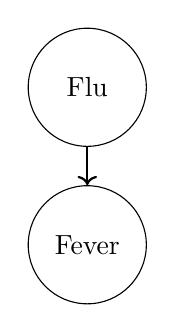
\begin{tikzpicture}[node distance=2cm]
    \node[draw, circle, minimum size=1.5cm] (flu) {Flu};
    \node[draw, circle, minimum size=1.5cm, below of=flu] (fever) {Fever};
    \draw[->, thick] (flu) -- (fever);
\end{tikzpicture}
\end{center}

\textbf{Conditional Probability Distributions:}

\textbf{Prior Probability of Flu:}
\begin{center}
\begin{tabular}{|c|c|}
\hline
Flu & Probability\\
\hline
No & 0.90\\
Yes & 0.10\\
\hline
\end{tabular}
\end{center}

\textbf{Conditional Probability of Fever given Flu:}
\begin{center}
\begin{tabular}{|c|c|c|}
\hline
Flu & Fever = No & Fever = Yes\\
\hline
No & 0.95 & 0.05\\
Yes & 0.10 & 0.90\\
\hline
\end{tabular}
\end{center}

\begin{algorithm}[H]
\caption{Bayesian Network Inference (Variable Elimination)}
\begin{algorithmic}[1]
\State \textbf{Input:} Bayesian Network $BN$, Query variable $X$, Evidence $E$
\State \textbf{Output:} $P(X|E)$
\State
\State Initialize factors from CPDs in $BN$
\State \textbf{for} each evidence variable $e_i \in E$ \textbf{do}
    \State \quad Restrict factors to observed values
\State \textbf{end for}
\State
\State elimination\_order $\gets$ ChooseOrdering$(BN, X, E)$
\State \textbf{for} each variable $V$ in elimination\_order \textbf{do}
    \State \quad factors\_with\_V $\gets$ factors containing $V$
    \State \quad new\_factor $\gets$ Product$(factors\_with\_V)$
    \State \quad new\_factor $\gets$ SumOut$(new\_factor, V)$
    \State \quad factors $\gets$ (factors $-$ factors\_with\_V) $\cup$ \{new\_factor\}
\State \textbf{end for}
\State
\State result $\gets$ Product$(factors)$
\State result $\gets$ Normalize$(result)$
\State \Return result
\end{algorithmic}
\end{algorithm}

\textbf{Inference Queries:}

\textbf{Query 1:} What is the probability of having flu given fever?
\begin{align*}
P(Flu=Yes|Fever=Yes) &= \frac{P(Fever=Yes|Flu=Yes) \cdot P(Flu=Yes)}{P(Fever=Yes)}\\
&= \frac{0.90 \times 0.10}{0.135}\\
&= 0.667 \text{ (66.7\%)}
\end{align*}

\textbf{Query 2:} What is the probability of having flu given no fever?
\begin{align*}
P(Flu=Yes|Fever=No) &= \frac{P(Fever=No|Flu=Yes) \cdot P(Flu=Yes)}{P(Fever=No)}\\
&= \frac{0.10 \times 0.10}{0.865}\\
&= 0.0116 \text{ (1.16\%)}
\end{align*}

\textbf{Interpretation:}
\begin{itemize}
    \item Observing fever significantly increases flu probability (from 10\% to 66.7\%)
    \item Absence of fever makes flu very unlikely (only 1.16\%)
    \item This demonstrates diagnostic reasoning using Bayesian inference
\end{itemize}

\textbf{Bayesian Network Factorization:}

A Bayesian Network encodes the joint probability distribution using the chain rule with conditional independence:

\begin{equation}
P(X_1, X_2, \ldots, X_n) = \prod_{i=1}^{n} P(X_i | \text{Parents}(X_i))
\end{equation}

\textbf{Bayes' Theorem - Foundation of Inference:}

\begin{equation}
P(H|E) = \frac{P(E|H) \cdot P(H)}{P(E)} = \frac{P(E|H) \cdot P(H)}{\sum_{h} P(E|h) \cdot P(h)}
\end{equation}

where $H$ is hypothesis, $E$ is evidence, $P(H)$ is prior, $P(E|H)$ is likelihood, $P(H|E)$ is posterior.

\textbf{D-Separation and Conditional Independence:}

Two sets of nodes $X$ and $Y$ are d-separated by set $Z$ if every undirected path between any node in $X$ and any node in $Y$ is blocked by $Z$. A path is blocked if:
\begin{itemize}
    \item There is a chain $A \rightarrow B \rightarrow C$ or fork $A \leftarrow B \rightarrow C$ where $B \in Z$
    \item There is a collider $A \rightarrow B \leftarrow C$ where $B \notin Z$ and no descendant of $B$ is in $Z$
\end{itemize}

If $X$ and $Y$ are d-separated by $Z$: $P(X|Y,Z) = P(X|Z)$ (conditional independence)

\textbf{Variable Elimination Complexity:}

Variable elimination algorithm complexity depends on induced width $w$:
\begin{equation}
\text{Time Complexity} = O(n \cdot k^{w+1})
\end{equation}
where $n$ = number of variables, $k$ = max domain size, $w$ = induced width.

\textbf{Markov Blanket:}

The Markov Blanket of node $X$ consists of: Parents of $X$, Children of $X$, and other parents of children of $X$ (co-parents). Given its Markov Blanket $MB(X)$: $X$ is independent of all other nodes.

\begin{figure}[H]
    \centering
    \includegraphics[width=\textwidth]{q4_bayesian_networks_enhanced.png}
    \caption{Bayesian Networks - Comprehensive Probabilistic Inference: (a) Flu-Fever diagnostic network DAG with 6 nodes (Season$\rightarrow$Flu$\rightarrow$Fever, Flu$\rightarrow$Cough, Flu$\rightarrow$Fatigue, Fever$\rightarrow$Headache) showing parent-child relationships, (b) Conditional Probability Distribution (CPD) tables displayed as heatmaps for all 6 variables with probability values color-coded, (c) Variable elimination inference trace showing factor operations (multiply, marginalize) across 4 steps, (d) Posterior probability distributions after evidence observation shown as grouped bar charts for Flu/Fever/Cough/Fatigue given observed Headache, (e) Belief propagation message passing visualization with 12 messages between nodes and convergence metrics, (f) Junction tree structure with 4 cliques and separator sets annotated, (g) Markov Blanket illustration for Flu node highlighting parents (Season), children (Fever, Cough, Fatigue), and co-parents (None), (h) D-separation analysis with 6 independence queries tested on network structure, (i) Sensitivity analysis tornado chart showing impact of CPD parameter variations on query P(Flu|Evidence), (j) Network comparison: Exact vs Approximate inference methods on bar chart (Variable Elimination, Junction Tree, Gibbs Sampling, Likelihood Weighting), (k) Information flow diagram with edge weights representing mutual information I(X;Y), (l) Query complexity scatter plot showing number of operations vs number of evidence nodes for different inference algorithms.}
    \label{fig:q4_bayes}
\end{figure}

%------------------------------------------------------------------------------
% Q5: Market Basket Analysis
%------------------------------------------------------------------------------
\subsection{Q5: Market Basket Analysis}

\subsubsection{Part (a): Market Basket Analysis and Significance}

\begin{definition}[Market Basket Analysis]
Market Basket Analysis (MBA) is a data mining technique used to discover patterns and relationships in large datasets by identifying items that frequently appear together in transactions. It is primarily used in retail to understand customer purchasing behavior.
\end{definition}

\textbf{Significance in Unsupervised Learning:}

Market Basket Analysis is a form of \textbf{association rule mining}, which belongs to unsupervised learning because:
\begin{itemize}
    \item \textbf{No Target Variable:} Does not predict a specific outcome
    \item \textbf{Pattern Discovery:} Finds hidden patterns in unlabeled data
    \item \textbf{Exploratory Analysis:} Reveals structure without prior assumptions
\end{itemize}

\textbf{Applications:}
\begin{enumerate}
    \item \textbf{Retail:} Product placement, cross-selling, promotions, inventory management
    \item \textbf{E-commerce:} Recommendation systems, bundle offers, personalized marketing
    \item \textbf{Healthcare:} Disease co-occurrence analysis, treatment effectiveness patterns
    \item \textbf{Banking:} Credit card fraud detection, customer service bundling
    \item \textbf{Telecommunications:} Service package optimization, churn prediction
    \item \textbf{Web Analytics:} Click-stream analysis, user behavior patterns
\end{enumerate}

\textbf{Historical Context:}

Market Basket Analysis gained prominence in the 1990s with the famous "beer and diapers" anecdote from retail analytics, though its formal foundations trace back to earlier work in data mining and statistics.

\textbf{The Beer and Diapers Story:}

While often cited as urban legend, this story illustrates the power of MBA:
\begin{itemize}
    \item Analysis supposedly revealed young fathers buying diapers also purchased beer
    \item Retailers placed beer near diapers, increasing sales
    \item Demonstrates unintuitive associations discoverable through data
    \item Highlights importance of actionable insights from patterns
\end{itemize}

\textbf{Fundamental Concepts in Association Rule Mining:}

\textbf{1. Itemsets:}
\begin{itemize}
    \item \textbf{1-itemset:} Single item, e.g., \{Bread\}
    \item \textbf{2-itemset:} Pair of items, e.g., \{Bread, Milk\}
    \item \textbf{k-itemset:} Set of $k$ items
    \item \textbf{Frequent itemset:} Itemset with support $\geq$ minimum threshold
\end{itemize}

\textbf{2. Association Rules:}

A rule has form $X \Rightarrow Y$ where:
\begin{itemize}
    \item $X$ is antecedent (left-hand side)
    \item $Y$ is consequent (right-hand side)
    \item $X \cap Y = \emptyset$ (disjoint sets)
\end{itemize}

\textbf{Quality Metrics Beyond Support, Confidence, Lift:}

\begin{enumerate}
    \item \textbf{Conviction:}
    \begin{equation}
    \text{conv}(X \Rightarrow Y) = \frac{1 - \text{supp}(Y)}{1 - \text{conf}(X \Rightarrow Y)}
    \end{equation}
    Measures dependency of consequent on antecedent. Ranges from 0 to $\infty$.

    \item \textbf{Leverage:}
    \begin{equation}
    \text{lev}(X \Rightarrow Y) = \text{supp}(X \cup Y) - \text{supp}(X) \times \text{supp}(Y)
    \end{equation}
    Difference between observed and expected frequency under independence.

    \item \textbf{Jaccard Index:}
    \begin{equation}
    J(X, Y) = \frac{|X \cap Y|}{|X \cup Y|} = \frac{\text{supp}(X \cup Y)}{\text{supp}(X) + \text{supp}(Y) - \text{supp}(X \cup Y)}
    \end{equation}
    Similarity measure between two itemsets.

    \item \textbf{Cosine Similarity:}
    \begin{equation}
    \cos(X, Y) = \frac{\text{supp}(X \cup Y)}{\sqrt{\text{supp}(X) \times \text{supp}(Y)}}
    \end{equation}

    \item \textbf{Kulczynski Measure:}
    \begin{equation}
    \text{Kulc}(X, Y) = \frac{1}{2}\left(\frac{\text{supp}(X \cup Y)}{\text{supp}(X)} + \frac{\text{supp}(X \cup Y)}{\text{supp}(Y)}\right)
    \end{equation}
    Average of conditional probabilities.

    \item \textbf{Imbalance Ratio:}
    \begin{equation}
    IR(X, Y) = \frac{|\text{supp}(X) - \text{supp}(Y)|}{\text{supp}(X) + \text{supp}(Y) - \text{supp}(X \cup Y)}
    \end{equation}
    Measures asymmetry between itemsets.
\end{enumerate}

\textbf{Interpretation Guidelines:}

\begin{center}
\begin{tabular}{|l|c|c|p{5cm}|}
\hline
\textbf{Metric} & \textbf{Range} & \textbf{Good Value} & \textbf{Interpretation}\\
\hline
Support & [0, 1] & $\geq$ 0.01 & Frequency of itemset\\
Confidence & [0, 1] & $\geq$ 0.5 & Reliability of rule\\
Lift & [0, $\infty$) & $> 1.0$ & Strength of association\\
Conviction & [0, $\infty$) & $> 1.5$ & Rule dependency\\
Leverage & [-1, 1] & $> 0$ & Practical significance\\
\hline
\end{tabular}
\end{center}

\textbf{The Apriori Algorithm: Detailed Mechanics}

The Apriori algorithm, developed by Agrawal and Srikant (1994), uses a level-wise search to discover frequent itemsets.

\textbf{Core Principle - Apriori Property:}
\begin{theorem}[Downward Closure Property]
If an itemset is frequent, then all of its subsets must also be frequent. Conversely, if an itemset is infrequent, all of its supersets must be infrequent.
\end{theorem}

Formally:
\begin{equation}
\forall X, Y: (X \subseteq Y) \Rightarrow (\text{supp}(X) \geq \text{supp}(Y))
\end{equation}

This anti-monotone property allows efficient pruning of the search space.

\textbf{Algorithm Steps:}

\begin{enumerate}
    \item \textbf{Scan 1:} Count support of all items (1-itemsets)
    \item \textbf{Generate:} $L_1$ = frequent 1-itemsets ($\text{supp} \geq \text{min\_supp}$)
    \item \textbf{Iterate for $k = 2, 3, ...$:}
    \begin{itemize}
        \item \textbf{Join Step:} Generate candidate $k$-itemsets $C_k$ from $L_{k-1}$
        \item \textbf{Prune Step:} Remove candidates with infrequent $(k-1)$-subsets
        \item \textbf{Scan:} Count support of candidates in $C_k$
        \item \textbf{Filter:} $L_k$ = frequent itemsets from $C_k$
    \end{itemize}
    \item \textbf{Terminate:} When $L_k = \emptyset$
    \item \textbf{Generate Rules:} From all frequent itemsets
\end{enumerate}

\textbf{Join Step Details:}

To generate $C_k$ from $L_{k-1}$:
\begin{equation}
C_k = \{X \cup Y : X, Y \in L_{k-1}, |X \cap Y| = k-2\}
\end{equation}

Example: If $L_2 = \{\{A,B\}, \{A,C\}, \{B,C\}\}$, then:
\begin{align}
\{A,B\} \cup \{A,C\} &= \{A,B,C\} \quad \text{(join on $A$)}\\
\{A,B\} \cup \{B,C\} &= \{A,B,C\} \quad \text{(join on $B$)}\\
\{A,C\} \cup \{B,C\} &= \{A,B,C\} \quad \text{(join on $C$)}\\
C_3 &= \{\{A,B,C\}\}
\end{align}

\textbf{Prune Step Details:}

For each candidate $c \in C_k$, check all $(k-1)$-subsets:
\begin{equation}
\forall s \subset c, |s| = k-1: \text{if } s \notin L_{k-1} \text{ then remove } c \text{ from } C_k
\end{equation}

\textbf{Complexity Analysis:}

\begin{itemize}
    \item \textbf{Candidate Generation:} $O(|L_{k-1}|^2)$ join operations
    \item \textbf{Subset Checking:} $O(|C_k| \times 2^k)$ for prune step
    \item \textbf{Database Scans:} $O(n \times m \times k)$ where:
    \begin{itemize}
        \item $n$ = number of transactions
        \item $m$ = number of candidates
        \item $k$ = itemset size
    \end{itemize}
    \item \textbf{Total:} $O(k_{max} \times n \times |C|_{avg})$ where $k_{max}$ is maximum itemset size
\end{itemize}

\textbf{Computational Challenges:}

\begin{enumerate}
    \item \textbf{Multiple Database Scans:} Each level $k$ requires full scan
    \item \textbf{Large Candidate Sets:} Combinatorial explosion
    \begin{itemize}
        \item With 100 items, potential $\binom{100}{2} = 4,950$ 2-itemsets
        \item With 1000 items, potential $\binom{1000}{2} = 499,500$ 2-itemsets
    \end{itemize}
    \item \textbf{Low Minimum Support:} More frequent itemsets $\Rightarrow$ more candidates
    \item \textbf{Memory Requirements:} All candidates must fit in memory
\end{enumerate}

\textbf{Optimization Techniques:}

\begin{enumerate}
    \item \textbf{Hash Tree for Candidate Counting:}
    \begin{itemize}
        \item Store candidates in hash tree structure
        \item Interior nodes contain hash tables
        \item Leaf nodes contain itemsets
        \item Reduces lookup from $O(m)$ to $O(\log m)$ average
        \item Hash function: $h(i) = i \mod \text{bucket\_size}$
    \end{itemize}

    \item \textbf{Transaction Projection:}
    \begin{itemize}
        \item For level $k$, only items in $L_{k-1}$ are relevant
        \item Project transactions to only frequent items
        \item Reduces transaction size progressively
        \item Example: $\{A, B, C, D, E\} \xrightarrow{\text{project}} \{A, B, C\}$ if only $A, B, C$ are frequent
    \end{itemize}

    \item \textbf{Dynamic Itemset Counting:}
    \begin{itemize}
        \item Start counting new candidates before completing current level
        \item Reduces number of database scans
        \item Trade-off: complexity vs. efficiency
    \end{itemize}

    \item \textbf{Sampling:}
    \begin{itemize}
        \item Mine frequent itemsets from sample of transactions
        \item Verify results on full database
        \item Sample size: $s = \frac{1}{\epsilon^2} \ln\frac{2}{\delta}$ for accuracy $\epsilon$ and confidence $1-\delta$
        \item Probabilistic guarantee: Found itemsets are frequent with probability $1-\delta$
    \end{itemize}

    \item \textbf{Partitioning:}
    \begin{itemize}
        \item Divide database into $p$ partitions
        \item Mine frequent itemsets in each partition
        \item Global frequent itemsets $\subseteq$ union of partition itemsets
        \item Only 2 database scans required
        \item Partition size: $\frac{n}{p}$ transactions per partition
    \end{itemize}
\end{enumerate}

\begin{example}[Grocery Store Analysis]
Transaction data from a grocery store:
\begin{itemize}
    \item Transaction 1: \{Milk, Bread, Butter\}
    \item Transaction 2: \{Bread, Diaper, Beer, Eggs\}
    \item Transaction 3: \{Milk, Diaper, Beer, Cola\}
    \item Transaction 4: \{Bread, Milk, Diaper, Beer\}
\end{itemize}

Pattern discovered: Customers who buy \{Diaper\} often buy \{Beer\}
\end{example}

\textbf{Business Benefits:}
\begin{itemize}
    \item Optimize product placement (put related items together)
    \item Design effective promotions (bundle frequently bought items)
    \item Manage inventory efficiently
    \item Understand customer preferences
    \item Increase sales through targeted marketing
\end{itemize}

\textbf{Worked Example: Apriori Algorithm Execution}

Consider a transaction database with minimum support = 40\% (2 out of 5 transactions):

\begin{center}
\begin{tabular}{|c|l|}
\hline
\textbf{TID} & \textbf{Items}\\
\hline
T1 & \{Milk, Bread, Butter\}\\
T2 & \{Milk, Bread, Cheese\}\\
T3 & \{Bread, Butter, Cheese\}\\
T4 & \{Milk, Bread, Butter, Cheese\}\\
T5 & \{Milk, Cheese\}\\
\hline
\end{tabular}
\end{center}

\textbf{Iteration 1: Find $L_1$}

Count support of 1-itemsets:
\begin{center}
\begin{tabular}{|c|c|c|}
\hline
\textbf{Itemset} & \textbf{Count} & \textbf{Support}\\
\hline
\{Milk\} & 4 & 80\%\\
\{Bread\} & 4 & 80\%\\
\{Butter\} & 3 & 60\%\\
\{Cheese\} & 4 & 80\%\\
\hline
\end{tabular}
\end{center}

All items meet minimum support: $L_1 = \{\{Milk\}, \{Bread\}, \{Butter\}, \{Cheese\}\}$

\textbf{Iteration 2: Find $L_2$}

Join Step: Generate $C_2 = \{\{M,B\}, \{M,Bu\}, \{M,C\}, \{B,Bu\}, \{B,C\}, \{Bu,C\}\}$

Count support:
\begin{center}
\begin{tabular}{|c|c|c|c|}
\hline
\textbf{Itemset} & \textbf{Count} & \textbf{Support} & \textbf{Frequent?}\\
\hline
\{Milk, Bread\} & 3 & 60\% & Yes\\
\{Milk, Butter\} & 2 & 40\% & Yes\\
\{Milk, Cheese\} & 3 & 60\% & Yes\\
\{Bread, Butter\} & 3 & 60\% & Yes\\
\{Bread, Cheese\} & 3 & 60\% & Yes\\
\{Butter, Cheese\} & 2 & 40\% & Yes\\
\hline
\end{tabular}
\end{center}

$L_2 = \{\{M,B\}, \{M,Bu\}, \{M,C\}, \{B,Bu\}, \{B,C\}, \{Bu,C\}\}$ (all 6 pairs)

\textbf{Iteration 3: Find $L_3$}

Join Step: Combine pairs sharing one item:
\begin{align}
\{M,B\} \cup \{M,Bu\} &= \{M,B,Bu\}\\
\{M,B\} \cup \{M,C\} &= \{M,B,C\}\\
\{M,Bu\} \cup \{M,C\} &= \{M,Bu,C\}\\
\{B,Bu\} \cup \{B,C\} &= \{B,Bu,C\}\\
\{M,B\} \cup \{B,Bu\} &= \{M,B,Bu\} \quad \text{(duplicate)}\\
\{M,B\} \cup \{B,C\} &= \{M,B,C\} \quad \text{(duplicate)}\\
&\vdots
\end{align}

After removing duplicates: $C_3 = \{\{M,B,Bu\}, \{M,B,C\}, \{M,Bu,C\}, \{B,Bu,C\}\}$

Prune Step: Check all 2-subsets are in $L_2$ (they are).

Count support:
\begin{center}
\begin{tabular}{|c|c|c|c|}
\hline
\textbf{Itemset} & \textbf{Count} & \textbf{Support} & \textbf{Frequent?}\\
\hline
\{M, B, Bu\} & 2 & 40\% & Yes\\
\{M, B, C\} & 2 & 40\% & Yes\\
\{M, Bu, C\} & 1 & 20\% & No\\
\{B, Bu, C\} & 2 & 40\% & Yes\\
\hline
\end{tabular}
\end{center}

$L_3 = \{\{M,B,Bu\}, \{M,B,C\}, \{B,Bu,C\}\}$

\textbf{Iteration 4: Find $L_4$}

Join Step: Only one candidate possible: $\{M,B,Bu,C\}$

Count: Support = 20\% (only T4) $<$ 40\% threshold

$L_4 = \emptyset$ $\Rightarrow$ Algorithm terminates

\textbf{Result:} All frequent itemsets = $L_1 \cup L_2 \cup L_3$ (13 itemsets total)

\textbf{Comparison with Alternative Algorithms:}

\begin{center}
\begin{tabular}{|p{2.5cm}|p{2.8cm}|p{2.8cm}|p{2.8cm}|p{2.8cm}|}
\hline
\textbf{Algorithm} & \textbf{Apriori} & \textbf{FP-Growth} & \textbf{Eclat} & \textbf{Deep Learning}\\
\hline
\textbf{Approach} & Level-wise breadth-first & Divide-and-conquer depth-first & Depth-first with vertical format & Neural embedding\\
\hline
\textbf{Data Structure} & Candidate hash tree & FP-tree (prefix tree) & TID-list (transaction IDs) & Embedding space\\
\hline
\textbf{Database Scans} & $k+1$ scans for max itemset size $k$ & 2 scans (build tree, mine) & 1 scan (load data) & Multiple epochs\\
\hline
\textbf{Candidate Generation} & Generate-and-test & No candidates (pattern growth) & No candidates (intersection) & Implicit (gradient descent)\\
\hline
\textbf{Memory} & Moderate (candidates) & High (tree structure) & Very high (TID-lists) & Moderate (embeddings)\\
\hline
\textbf{Speed} & Slow for low support & Fast & Very fast for sparse data & Slow (training)\\
\hline
\textbf{Scalability} & Poor (many scans) & Good (2 scans) & Good (1 scan) & Excellent (batch)\\
\hline
\textbf{Dense Data} & Poor & Good & Poor (large TID-lists) & Good\\
\hline
\textbf{Sparse Data} & Moderate & Good & Excellent & Moderate\\
\hline
\textbf{Interpretability} & Excellent (explicit rules) & Excellent (explicit rules) & Excellent (explicit rules) & Poor (black box)\\
\hline
\textbf{Complexity} & $O(2^n)$ worst & $O(n \cdot |FP|)$ & $O(n \cdot m^2)$ & $O(e \cdot b \cdot n)$\\
\hline
\textbf{Best For} & Small datasets, teaching & Large datasets & Vertical databases & Recommendations\\
\hline
\textbf{Invented} & 1994 (Agrawal) & 2000 (Han) & 1997 (Zaki) & 2010s\\
\hline
\end{tabular}
\end{center}

Where: $n$ = transactions, $m$ = items, $|FP|$ = FP-tree size, $e$ = epochs, $b$ = batch size

\subsubsection{Part (b): Association Rule Mining Metrics}

Association rules have the form: $X \Rightarrow Y$ (if X then Y)

\textbf{Key Metrics:}

\textbf{1. Support:}

Support measures how frequently an itemset appears in the dataset.

\begin{definition}[Support]
\begin{equation}
Support(X) = \frac{\text{Number of transactions containing } X}{\text{Total number of transactions}}
\end{equation}

For a rule $X \Rightarrow Y$:
\begin{equation}
Support(X \Rightarrow Y) = \frac{\text{Transactions containing both } X \text{ and } Y}{\text{Total transactions}}
\end{equation}
\end{definition}

\textbf{Interpretation:} High support indicates the itemset is frequently purchased together.

\textbf{2. Confidence:}

Confidence measures how often Y appears in transactions that contain X.

\begin{definition}[Confidence]
\begin{equation}
Confidence(X \Rightarrow Y) = \frac{Support(X \cup Y)}{Support(X)} = P(Y|X)
\end{equation}
\end{definition}

\textbf{Interpretation:} High confidence indicates a strong association; if X is purchased, Y is likely purchased too.

\textbf{3. Lift:}

Lift measures how much more likely Y is purchased when X is purchased, compared to Y being purchased independently.

\begin{definition}[Lift]
\begin{equation}
Lift(X \Rightarrow Y) = \frac{Support(X \cup Y)}{Support(X) \times Support(Y)} = \frac{P(Y|X)}{P(Y)}
\end{equation}
\end{definition}

\textbf{Interpretation:}
\begin{itemize}
    \item Lift $>$ 1: Positive correlation (X and Y occur together more than expected)
    \item Lift $=$ 1: Independence (no correlation)
    \item Lift $<$ 1: Negative correlation (X and Y rarely occur together)
\end{itemize}

\begin{algorithm}[H]
\caption{Apriori Algorithm for Association Rule Mining}
\begin{algorithmic}[1]
\State \textbf{Input:} Transaction database $D$, minimum support $min\_sup$, minimum confidence $min\_conf$
\State \textbf{Output:} Set of association rules
\State
\State $L_1 \gets$ \{frequent 1-itemsets with support $\geq min\_sup$\}
\State $k \gets 2$
\While{$L_{k-1} \neq \emptyset$}
    \State $C_k \gets$ CandidateGeneration$(L_{k-1})$ \Comment{Generate candidates}
    \For{each transaction $t \in D$}
        \State $C_t \gets$ Subset$(C_k, t)$ \Comment{Candidates in transaction}
        \For{each candidate $c \in C_t$}
            \State $c.count \gets c.count + 1$
        \EndFor
    \EndFor
    \State $L_k \gets$ \{$c \in C_k | c.count/|D| \geq min\_sup$\}
    \State $k \gets k + 1$
\EndWhile
\State
\State $L \gets \bigcup_k L_k$ \Comment{All frequent itemsets}
\State
\State \textbf{Generate Rules:}
\For{each frequent itemset $l \in L, |l| \geq 2$}
    \For{each non-empty subset $s \subset l$}
        \State $rule \gets s \Rightarrow (l - s)$
        \State $conf \gets Support(l) / Support(s)$
        \If{$conf \geq min\_conf$}
            \State Output rule with support, confidence, lift
        \EndIf
    \EndFor
\EndFor
\end{algorithmic}
\end{algorithm}

\begin{example}[Calculating Metrics]
Transaction database with 10 transactions:
\begin{itemize}
    \item Support(\{Bread\}) = 7/10 = 0.70
    \item Support(\{Milk\}) = 6/10 = 0.60
    \item Support(\{Bread, Milk\}) = 5/10 = 0.50
\end{itemize}

For rule: Bread $\Rightarrow$ Milk:
\begin{itemize}
    \item Confidence = 0.50/0.70 = 0.714 (71.4\%)
    \item Lift = 0.50/(0.70 $\times$ 0.60) = 1.19
\end{itemize}

\textbf{Interpretation:} When bread is purchased, milk is bought 71.4\% of the time, which is 1.19 times more than if purchases were independent.
\end{example}

\textbf{Apriori Algorithm - Anti-Monotone Property:}

\begin{theorem}[Anti-Monotonicity]
If an itemset $I$ is infrequent, then all supersets of $I$ are also infrequent.
\end{theorem}

Mathematically: If $\text{support}(I) < \text{min\_support}$ then $\forall S \supseteq I: \text{support}(S) < \text{min\_support}$

This property allows pruning the search space effectively.

\textbf{Key Metrics Mathematical Definitions:}

\begin{align}
\text{Support}(X \Rightarrow Y) &= \frac{\text{transactions containing } X \cup Y}{\text{total transactions}} = P(X \cap Y)\\
\text{Confidence}(X \Rightarrow Y) &= \frac{\text{support}(X \cup Y)}{\text{support}(X)} = P(Y|X)\\
\text{Lift}(X \Rightarrow Y) &= \frac{\text{confidence}(X \Rightarrow Y)}{\text{support}(Y)} = \frac{P(X \cap Y)}{P(X) \cdot P(Y)}
\end{align}

\textbf{Lift Interpretation:}
\begin{itemize}
    \item Lift $> 1$: Positive correlation (items purchased together more than expected)
    \item Lift $= 1$: No correlation (items independent)
    \item Lift $< 1$: Negative correlation (items purchased together less than expected)
\end{itemize}

\textbf{Conviction Metric:}

Conviction measures rule implication strength:
\begin{equation}
\text{Conviction}(X \Rightarrow Y) = \frac{1 - \text{support}(Y)}{1 - \text{confidence}(X \Rightarrow Y)} = \frac{P(X)P(\neg Y)}{P(X \cap \neg Y)}
\end{equation}

\textbf{Itemset Lattice Structure:}

The search space forms a lattice with:
\begin{itemize}
    \item \textbf{Bottom:} Empty set $\emptyset$
    \item \textbf{Level $k$:} All itemsets of size $k$
    \item \textbf{Edges:} Connect itemsets differing by one item
    \item \textbf{Size:} $\sum_{k=0}^{n} \binom{n}{k} = 2^n$ possible itemsets for $n$ items
\end{itemize}

\begin{figure}[H]
    \centering
    \includegraphics[width=\textwidth]{q5_market_basket_analysis_enhanced.png}
    \caption{Market Basket Analysis - Comprehensive Association Rule Mining: (a) Transaction-item matrix heatmap showing 100 transactions across 20 items with purchase indicators (1=purchased, 0=not purchased), (b) Frequent itemset lattice visualization showing hierarchical structure from level 0 (empty) to level 4 with 45 frequent itemsets connected by subset relationships, (c) Association rules network graph with 50 rules displayed as directed edges, nodes sized by item frequency, edges colored by lift value (red=high, blue=low), (d) Support-Confidence-Lift 3D scatter plot with 50 rules as points, bubble size representing interest measure, color gradient showing conviction values, (e) Item frequency distribution bar chart showing top 20 items ranked by support percentage, (f) Rule quality metrics spider chart comparing top 10 rules across 6 dimensions (support, confidence, lift, conviction, cosine, Jaccard), (g) Temporal association patterns line plot showing rule confidence evolution across 5 time windows, (h) Product affinity heatmap matrix showing lift values between all item pairs with hierarchical clustering dendrogram, (i) Cross-selling opportunity matrix identifying high-lift item combinations for recommendation, (j) Rule pruning comparison bars showing number of rules at different confidence thresholds (50\%, 60\%, 70\%, 80\%, 90\%), (k) Apriori algorithm performance metrics (execution time, memory usage, candidate generation) across different minimum support levels, (l) Market basket size distribution histogram with overlay curve showing average basket size and standard deviation.}
    \label{fig:q5_mba}
\end{figure}

%------------------------------------------------------------------------------
% Q6: Neural Networks
%------------------------------------------------------------------------------
\subsection{Q6: Neural Networks}

\subsubsection{Part (a): Perceptron}

\begin{definition}[Perceptron]
A perceptron is the simplest form of an artificial neural network, consisting of a single neuron that performs binary classification by computing a weighted sum of inputs and applying a step activation function.
\end{definition}

\textbf{Perceptron Architecture:}

\begin{center}
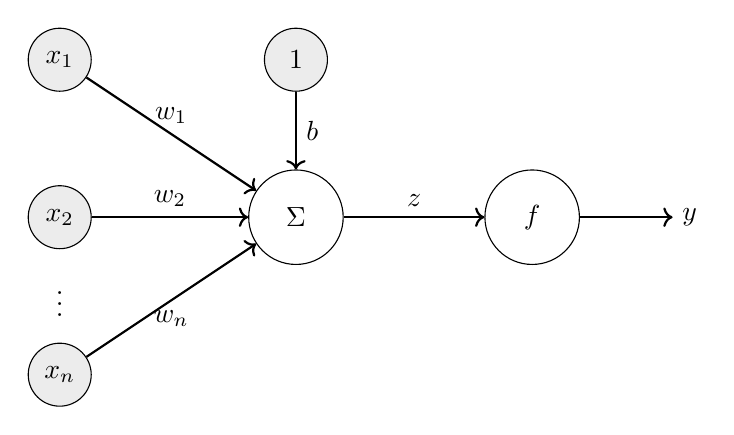
\begin{tikzpicture}[
    node distance=2cm,
    neuron/.style={circle, draw, minimum size=1.2cm},
    input/.style={circle, draw, minimum size=0.8cm, fill=lightgray!30}
]
    % Input nodes
    \node[input] (x1) at (0,2) {$x_1$};
    \node[input] (x2) at (0,0) {$x_2$};
    \node[input] (xn) at (0,-2) {$x_n$};

    % Hidden representation
    \node at (0,-1) {$\vdots$};

    % Weighted sum node
    \node[neuron] (sum) at (3,0) {$\Sigma$};

    % Activation node
    \node[neuron] (act) at (6,0) {$f$};

    % Output
    \node (output) at (8,0) {$y$};

    % Connections
    \draw[->, thick] (x1) -- node[above] {$w_1$} (sum);
    \draw[->, thick] (x2) -- node[above] {$w_2$} (sum);
    \draw[->, thick] (xn) -- node[below] {$w_n$} (sum);

    \draw[->, thick] (sum) -- node[above] {$z$} (act);
    \draw[->, thick] (act) -- (output);

    % Bias
    \node[input] (bias) at (3,2) {$1$};
    \draw[->, thick] (bias) -- node[right] {$b$} (sum);
\end{tikzpicture}
\end{center}

\textbf{Mathematical Model:}

\textbf{1. Weighted Sum:}
\begin{equation}
z = \sum_{i=1}^{n} w_i x_i + b = \mathbf{w}^T \mathbf{x} + b
\end{equation}

where:
\begin{itemize}
    \item $x_i$ are input features
    \item $w_i$ are weights
    \item $b$ is the bias term
\end{itemize}

\textbf{2. Activation Function (Step Function):}
\begin{equation}
y = f(z) = \begin{cases}
1 & \text{if } z \geq 0\\
0 & \text{if } z < 0
\end{cases}
\end{equation}

\textbf{3. Learning Rule (Perceptron Learning Algorithm):}

For each training example $(\mathbf{x}, t)$ where $t$ is the target:
\begin{align}
\text{Prediction: } &\hat{y} = f(\mathbf{w}^T \mathbf{x} + b)\\
\text{Error: } &e = t - \hat{y}\\
\text{Weight Update: } &w_i \gets w_i + \eta \cdot e \cdot x_i\\
\text{Bias Update: } &b \gets b + \eta \cdot e
\end{align}

where $\eta$ is the learning rate.

\begin{algorithm}[H]
\caption{Perceptron Training Algorithm}
\begin{algorithmic}[1]
\State \textbf{Input:} Training data $\{(\mathbf{x}^{(i)}, t^{(i)})\}_{i=1}^{m}$, learning rate $\eta$, epochs $T$
\State \textbf{Output:} Learned weights $\mathbf{w}$ and bias $b$
\State
\State Initialize $\mathbf{w} \gets \mathbf{0}$, $b \gets 0$
\For{epoch $= 1$ to $T$}
    \State $errors \gets 0$
    \For{each training example $(\mathbf{x}, t)$}
        \State $z \gets \mathbf{w}^T \mathbf{x} + b$
        \State $\hat{y} \gets$ Step$(z)$ \Comment{Apply activation}
        \State $e \gets t - \hat{y}$
        \State $\mathbf{w} \gets \mathbf{w} + \eta \cdot e \cdot \mathbf{x}$
        \State $b \gets b + \eta \cdot e$
        \State $errors \gets errors + |e|$
    \EndFor
    \If{$errors = 0$}
        \State \textbf{break} \Comment{Converged}
    \EndIf
\EndFor
\State \Return $\mathbf{w}, b$
\end{algorithmic}
\end{algorithm}

\textbf{Properties:}
\begin{itemize}
    \item \textbf{Convergence:} Guaranteed to converge for linearly separable data
    \item \textbf{Limitation:} Cannot learn non-linearly separable problems (e.g., XOR)
    \item \textbf{Geometric Interpretation:} Learns a hyperplane separating classes
\end{itemize}

\textbf{Historical Context - The Perceptron Controversy:}

\begin{enumerate}
    \item \textbf{1957:} Frank Rosenblatt invents the perceptron at Cornell Aeronautical Laboratory
    \item \textbf{1958:} First hardware implementation - Mark I Perceptron
    \item \textbf{Initial Excitement:} Media hype about "embryo of electronic computer"
    \item \textbf{1969:} Minsky and Papert publish "Perceptrons" book
    \begin{itemize}
        \item Proved single-layer perceptrons cannot solve XOR problem
        \item Showed limitations for non-linearly separable data
        \item Led to first "AI Winter" with reduced funding
    \end{itemize}
    \item \textbf{1980s:} Revival with multi-layer networks and backpropagation
    \item \textbf{Modern View:} Perceptron as building block for deep learning
\end{enumerate}

\textbf{XOR Problem - Perceptron's Fundamental Limitation:}

The XOR function demonstrates non-linear separability:

\begin{center}
\begin{tabular}{|c|c|c|}
\hline
$x_1$ & $x_2$ & XOR Output\\
\hline
0 & 0 & 0\\
0 & 1 & 1\\
1 & 0 & 1\\
1 & 1 & 0\\
\hline
\end{tabular}
\end{center}

\textbf{Proof of XOR Non-Linear Separability:}

Assume decision boundary: $w_1 x_1 + w_2 x_2 + b = 0$

For XOR to be learnable by single perceptron:
\begin{align}
w_1(0) + w_2(0) + b &< 0 \quad \text{(output 0)}\\
w_1(0) + w_2(1) + b &> 0 \quad \text{(output 1)}\\
w_1(1) + w_2(0) + b &> 0 \quad \text{(output 1)}\\
w_1(1) + w_2(1) + b &< 0 \quad \text{(output 0)}
\end{align}

From equations (2) and (3): $w_2 + b > 0$ and $w_1 + b > 0$

Therefore: $w_1 + w_2 + b > w_1 + b > 0$ and $w_1 + w_2 + b > w_2 + b > 0$

This contradicts equation (4): $w_1 + w_2 + b < 0$

\textbf{Conclusion:} No linear boundary exists $\Rightarrow$ Single perceptron cannot solve XOR

\textbf{Solution:} Multi-layer network with hidden layers can solve XOR

\textbf{Perceptron Convergence Theorem:}

\begin{theorem}[Novikoff, 1962]
If training data is linearly separable with margin $\gamma > 0$, the perceptron algorithm converges in at most $\frac{R^2}{\gamma^2}$ updates, where $R$ is the maximum norm of input vectors: $R = \max_i \|\mathbf{x}^{(i)}\|$.
\end{theorem}

\textbf{Proof Sketch:}

Let $\mathbf{w}^*$ be optimal separating hyperplane with $\|\mathbf{w}^*\| = 1$ and margin $\gamma$.

After $k$ mistakes, weight vector is $\mathbf{w}^{(k)} = \mathbf{w}^{(k-1)} + y^{(i)}\mathbf{x}^{(i)}$

\textbf{Lower bound on $\mathbf{w}^* \cdot \mathbf{w}^{(k)}$:}
\begin{align}
\mathbf{w}^* \cdot \mathbf{w}^{(k)} &= \mathbf{w}^* \cdot (\mathbf{w}^{(k-1)} + y^{(i)}\mathbf{x}^{(i)})\\
&= \mathbf{w}^* \cdot \mathbf{w}^{(k-1)} + y^{(i)}(\mathbf{w}^* \cdot \mathbf{x}^{(i)})\\
&\geq \mathbf{w}^* \cdot \mathbf{w}^{(k-1)} + \gamma\\
&\geq k\gamma \quad \text{(by induction)}
\end{align}

\textbf{Upper bound on $\|\mathbf{w}^{(k)}\|^2$:}
\begin{align}
\|\mathbf{w}^{(k)}\|^2 &= \|\mathbf{w}^{(k-1)} + y^{(i)}\mathbf{x}^{(i)}\|^2\\
&= \|\mathbf{w}^{(k-1)}\|^2 + 2y^{(i)}\mathbf{w}^{(k-1)} \cdot \mathbf{x}^{(i)} + \|\mathbf{x}^{(i)}\|^2\\
&\leq \|\mathbf{w}^{(k-1)}\|^2 + R^2 \quad \text{(mistake implies } 2y^{(i)}\mathbf{w}^{(k-1)} \cdot \mathbf{x}^{(i)} \leq 0\text{)}\\
&\leq kR^2 \quad \text{(by induction)}
\end{align}

Combining bounds using Cauchy-Schwarz:
\begin{equation}
k\gamma \leq \mathbf{w}^* \cdot \mathbf{w}^{(k)} \leq \|\mathbf{w}^*\| \cdot \|\mathbf{w}^{(k)}\| = \|\mathbf{w}^{(k)}\| \leq \sqrt{kR^2} = \sqrt{k}R
\end{equation}

Therefore: $k\gamma \leq \sqrt{k}R \Rightarrow k \leq \frac{R^2}{\gamma^2}$

\textbf{Modern Variants of Perceptron:}

\begin{enumerate}
    \item \textbf{Averaged Perceptron:} Returns average of all weight vectors during training
    \begin{equation}
    \mathbf{w}_{\text{avg}} = \frac{1}{T \cdot m} \sum_{t=1}^{T} \sum_{i=1}^{m} \mathbf{w}^{(t,i)}
    \end{equation}
    Improves generalization, commonly used in NLP

    \item \textbf{Voted Perceptron:} Keeps distinct weight vectors with vote counts

    \item \textbf{Kernel Perceptron:} Uses kernel trick for non-linear decision boundaries
    \begin{equation}
    f(\mathbf{x}) = \text{sign}\left(\sum_{i=1}^{m} \alpha_i y^{(i)} K(\mathbf{x}^{(i)}, \mathbf{x}) + b\right)
    \end{equation}
    where $K(\cdot, \cdot)$ is kernel function (RBF, polynomial, etc.)

    \item \textbf{Passive-Aggressive Algorithm:} Variant for online learning with margins
\end{enumerate}

\subsubsection{Part (b): Backpropagation Algorithm}

\begin{definition}[Backpropagation]
Backpropagation is a supervised learning algorithm used to train multi-layer neural networks by computing gradients of the loss function with respect to weights using the chain rule, then updating weights to minimize the loss.
\end{definition}

\textbf{Multi-Layer Neural Network Architecture:}

\begin{center}
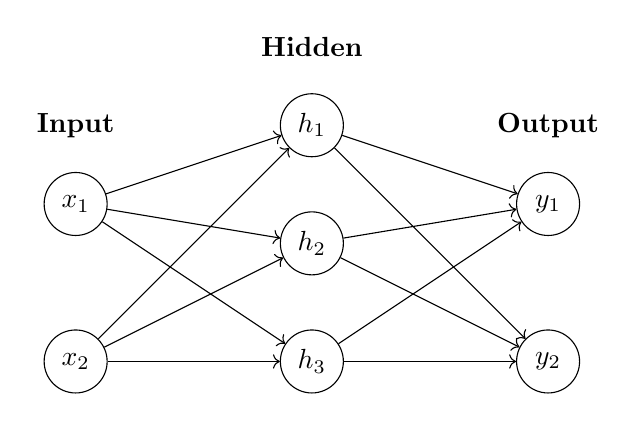
\begin{tikzpicture}[
    node distance=1.5cm and 2.5cm,
    neuron/.style={circle, draw, minimum size=0.8cm},
    layer/.style={rectangle, draw=none}
]
    % Input layer
    \node[neuron] (i1) at (0,2) {$x_1$};
    \node[neuron] (i2) at (0,0) {$x_2$};
    \node[layer] at (0,3) {\textbf{Input}};

    % Hidden layer
    \node[neuron] (h1) at (3,3) {$h_1$};
    \node[neuron] (h2) at (3,1.5) {$h_2$};
    \node[neuron] (h3) at (3,0) {$h_3$};
    \node[layer] at (3,4) {\textbf{Hidden}};

    % Output layer
    \node[neuron] (o1) at (6,2) {$y_1$};
    \node[neuron] (o2) at (6,0) {$y_2$};
    \node[layer] at (6,3) {\textbf{Output}};

    % Connections (input to hidden)
    \foreach \i in {1,2}
        \foreach \h in {1,2,3}
            \draw[->, thin] (i\i) -- (h\h);

    % Connections (hidden to output)
    \foreach \h in {1,2,3}
        \foreach \o in {1,2}
            \draw[->, thin] (h\h) -- (o\o);
\end{tikzpicture}
\end{center}

\textbf{Algorithm Components:}

\textbf{1. Forward Pass:}

Compute outputs layer by layer:
\begin{align}
\text{Hidden layer: } &h_j = \sigma\left(\sum_i w_{ij}^{(1)} x_i + b_j^{(1)}\right)\\
\text{Output layer: } &y_k = \sigma\left(\sum_j w_{jk}^{(2)} h_j + b_k^{(2)}\right)
\end{align}

where $\sigma$ is an activation function (e.g., sigmoid, ReLU).

\textbf{2. Loss Calculation:}

For regression: $L = \frac{1}{2}\sum_k (t_k - y_k)^2$ (Mean Squared Error)\\
For classification: $L = -\sum_k t_k \log(y_k)$ (Cross-Entropy)

\textbf{3. Backward Pass (Detailed Derivation):}

The goal is to compute $\frac{\partial L}{\partial w}$ for all weights to perform gradient descent.

\textbf{Notation:}
\begin{itemize}
    \item $z_j^{(l)} = \sum_i w_{ij}^{(l)} a_i^{(l-1)} + b_j^{(l)}$ (pre-activation)
    \item $a_j^{(l)} = \sigma(z_j^{(l)})$ (activation)
    \item $\delta_j^{(l)} = \frac{\partial L}{\partial z_j^{(l)}}$ (error signal)
    \item $L$ = loss function
    \item $l$ = layer index
\end{itemize}

\textbf{Step 1: Output Layer Error}

For output layer $L$ with target $t$ and output $a^{(L)}$:

\begin{align}
\delta_j^{(L)} &= \frac{\partial L}{\partial z_j^{(L)}}\\
&= \frac{\partial L}{\partial a_j^{(L)}} \cdot \frac{\partial a_j^{(L)}}{\partial z_j^{(L)}} \quad \text{(Chain rule)}\\
&= \frac{\partial L}{\partial a_j^{(L)}} \cdot \sigma'(z_j^{(L)})
\end{align}

For MSE loss: $L = \frac{1}{2}\sum_k (t_k - a_k^{(L)})^2$
\begin{equation}
\delta_j^{(L)} = (a_j^{(L)} - t_j) \cdot \sigma'(z_j^{(L)})
\end{equation}

For cross-entropy with softmax: $L = -\sum_k t_k \log(a_k^{(L)})$
\begin{equation}
\delta_j^{(L)} = a_j^{(L)} - t_j \quad \text{(simplified form)}
\end{equation}

\textbf{Step 2: Backpropagate Error to Hidden Layers}

For hidden layer $l$ (working backwards from output):

\begin{align}
\delta_j^{(l)} &= \frac{\partial L}{\partial z_j^{(l)}}\\
&= \sum_k \frac{\partial L}{\partial z_k^{(l+1)}} \cdot \frac{\partial z_k^{(l+1)}}{\partial a_j^{(l)}} \cdot \frac{\partial a_j^{(l)}}{\partial z_j^{(l)}}\\
&= \sum_k \delta_k^{(l+1)} \cdot w_{jk}^{(l+1)} \cdot \sigma'(z_j^{(l)})\\
&= \sigma'(z_j^{(l)}) \sum_k w_{jk}^{(l+1)} \delta_k^{(l+1)}
\end{align}

\textbf{Matrix Form:}
\begin{equation}
\boldsymbol{\delta}^{(l)} = (\mathbf{W}^{(l+1)})^T \boldsymbol{\delta}^{(l+1)} \odot \sigma'(\mathbf{z}^{(l)})
\end{equation}

where $\odot$ denotes element-wise multiplication (Hadamard product).

\textbf{Step 3: Compute Weight Gradients}

Once we have error signals $\delta_j^{(l)}$ for all neurons:

\begin{align}
\frac{\partial L}{\partial w_{ij}^{(l)}} &= \frac{\partial L}{\partial z_j^{(l)}} \cdot \frac{\partial z_j^{(l)}}{\partial w_{ij}^{(l)}}\\
&= \delta_j^{(l)} \cdot a_i^{(l-1)}
\end{align}

\begin{align}
\frac{\partial L}{\partial b_j^{(l)}} &= \frac{\partial L}{\partial z_j^{(l)}} \cdot \frac{\partial z_j^{(l)}}{\partial b_j^{(l)}}\\
&= \delta_j^{(l)} \cdot 1 = \delta_j^{(l)}
\end{align}

\textbf{Matrix Form:}
\begin{equation}
\frac{\partial L}{\partial \mathbf{W}^{(l)}} = \boldsymbol{\delta}^{(l)} (\mathbf{a}^{(l-1)})^T
\end{equation}

\textbf{Step 4: Update Weights}

Using gradient descent:
\begin{align}
w_{ij}^{(l)} &\gets w_{ij}^{(l)} - \eta \frac{\partial L}{\partial w_{ij}^{(l)}}\\
b_j^{(l)} &\gets b_j^{(l)} - \eta \frac{\partial L}{\partial b_j^{(l)}}
\end{align}

where $\eta$ is the learning rate.

\textbf{Complete Backpropagation Algorithm Summary:}

\begin{enumerate}
    \item \textbf{Forward Pass:} Compute all activations $a^{(l)}$ for $l = 1, ..., L$
    \item \textbf{Output Error:} Compute $\boldsymbol{\delta}^{(L)} = \nabla_{a^{(L)}} L \odot \sigma'(\mathbf{z}^{(L)})$
    \item \textbf{Backpropagate:} For $l = L-1, ..., 1$:
    \begin{equation}
    \boldsymbol{\delta}^{(l)} = (\mathbf{W}^{(l+1)})^T \boldsymbol{\delta}^{(l+1)} \odot \sigma'(\mathbf{z}^{(l)})
    \end{equation}
    \item \textbf{Gradients:} Compute $\frac{\partial L}{\partial \mathbf{W}^{(l)}} = \boldsymbol{\delta}^{(l)} (\mathbf{a}^{(l-1)})^T$
    \item \textbf{Update:} $\mathbf{W}^{(l)} \gets \mathbf{W}^{(l)} - \eta \frac{\partial L}{\partial \mathbf{W}^{(l)}}$
\end{enumerate}

\textbf{Concrete Example: 2-2-1 Network for XOR}

Network: 2 inputs $\rightarrow$ 2 hidden $\rightarrow$ 1 output

\textbf{Forward Pass Example:}

Input: $\mathbf{x} = [1, 0]^T$, Target: $t = 1$

Layer 1 (Input $\rightarrow$ Hidden):
\begin{align}
z_1^{(1)} &= w_{11}^{(1)} \cdot 1 + w_{21}^{(1)} \cdot 0 + b_1^{(1)} = 0.5 \cdot 1 + 0.3 \cdot 0 + 0.1 = 0.6\\
a_1^{(1)} &= \sigma(0.6) = \frac{1}{1+e^{-0.6}} = 0.646\\
z_2^{(1)} &= w_{12}^{(1)} \cdot 1 + w_{22}^{(1)} \cdot 0 + b_2^{(1)} = 0.4 \cdot 1 + 0.6 \cdot 0 - 0.2 = 0.2\\
a_2^{(1)} &= \sigma(0.2) = 0.550
\end{align}

Layer 2 (Hidden $\rightarrow$ Output):
\begin{align}
z_1^{(2)} &= w_{11}^{(2)} a_1^{(1)} + w_{21}^{(2)} a_2^{(1)} + b_1^{(2)}\\
&= 0.7 \cdot 0.646 + 0.8 \cdot 0.550 + 0.15 = 1.042\\
a_1^{(2)} &= \sigma(1.042) = 0.739
\end{align}

Loss: $L = \frac{1}{2}(t - a_1^{(2)})^2 = \frac{1}{2}(1 - 0.739)^2 = 0.034$

\textbf{Backward Pass Example:}

Output error:
\begin{align}
\delta_1^{(2)} &= (a_1^{(2)} - t) \cdot \sigma'(z_1^{(2)})\\
&= (0.739 - 1) \cdot (0.739 \cdot (1-0.739))\\
&= -0.261 \cdot 0.193 = -0.050
\end{align}

Hidden layer errors:
\begin{align}
\delta_1^{(1)} &= w_{11}^{(2)} \delta_1^{(2)} \cdot \sigma'(z_1^{(1)})\\
&= 0.7 \cdot (-0.050) \cdot (0.646 \cdot 0.354) = -0.008\\
\delta_2^{(1)} &= w_{21}^{(2)} \delta_1^{(2)} \cdot \sigma'(z_2^{(1)})\\
&= 0.8 \cdot (-0.050) \cdot (0.550 \cdot 0.450) = -0.010
\end{align}

Weight gradients (Layer 2):
\begin{align}
\frac{\partial L}{\partial w_{11}^{(2)}} &= \delta_1^{(2)} \cdot a_1^{(1)} = -0.050 \cdot 0.646 = -0.032\\
\frac{\partial L}{\partial w_{21}^{(2)}} &= \delta_1^{(2)} \cdot a_2^{(1)} = -0.050 \cdot 0.550 = -0.028
\end{align}

Weight updates (with $\eta = 0.1$):
\begin{align}
w_{11}^{(2)} &\gets 0.7 - 0.1 \cdot (-0.032) = 0.703\\
w_{21}^{(2)} &\gets 0.8 - 0.1 \cdot (-0.028) = 0.803
\end{align}

\textbf{3. Backward Pass (Summary):}

Compute gradients using chain rule:

\textbf{Output layer:}
\begin{equation}
\delta_k^{(output)} = \frac{\partial L}{\partial y_k} \cdot \sigma'(z_k)
\end{equation}

\textbf{Hidden layer:}
\begin{equation}
\delta_j^{(hidden)} = \left(\sum_k w_{jk}^{(2)} \delta_k^{(output)}\right) \cdot \sigma'(z_j)
\end{equation}

\textbf{4. Weight Update:}

\begin{align}
w_{jk}^{(2)} &\gets w_{jk}^{(2)} - \eta \frac{\partial L}{\partial w_{jk}^{(2)}} = w_{jk}^{(2)} - \eta \cdot \delta_k^{(output)} \cdot h_j\\
w_{ij}^{(1)} &\gets w_{ij}^{(1)} - \eta \frac{\partial L}{\partial w_{ij}^{(1)}} = w_{ij}^{(1)} - \eta \cdot \delta_j^{(hidden)} \cdot x_i
\end{align}

\begin{algorithm}[H]
\caption{Backpropagation Algorithm}
\begin{algorithmic}[1]
\State \textbf{Input:} Training data $\{(\mathbf{x}^{(i)}, \mathbf{t}^{(i)})\}$, learning rate $\eta$, epochs $T$
\State \textbf{Output:} Trained network weights
\State
\State Initialize all weights randomly
\For{epoch $= 1$ to $T$}
    \For{each training example $(\mathbf{x}, \mathbf{t})$}
        \State \textbf{// Forward Pass}
        \For{each layer $l$ from input to output}
            \State Compute activations: $\mathbf{a}^{(l)} = \sigma(\mathbf{W}^{(l)} \mathbf{a}^{(l-1)} + \mathbf{b}^{(l)})$
        \EndFor
        \State
        \State \textbf{// Compute Loss}
        \State $L \gets$ Loss$(\mathbf{y}, \mathbf{t})$
        \State
        \State \textbf{// Backward Pass}
        \State Compute output layer error: $\boldsymbol{\delta}^{(output)} \gets \nabla_{\mathbf{y}} L \odot \sigma'(\mathbf{z}^{(output)})$
        \For{each hidden layer $l$ from output to input}
            \State $\boldsymbol{\delta}^{(l)} \gets (\mathbf{W}^{(l+1)})^T \boldsymbol{\delta}^{(l+1)} \odot \sigma'(\mathbf{z}^{(l)})$
        \EndFor
        \State
        \State \textbf{// Update Weights}
        \For{each layer $l$}
            \State $\mathbf{W}^{(l)} \gets \mathbf{W}^{(l)} - \eta \cdot \boldsymbol{\delta}^{(l)} (\mathbf{a}^{(l-1)})^T$
            \State $\mathbf{b}^{(l)} \gets \mathbf{b}^{(l)} - \eta \cdot \boldsymbol{\delta}^{(l)}$
        \EndFor
    \EndFor
\EndFor
\end{algorithmic}
\end{algorithm}

\textbf{Key Advantages:}
\begin{itemize}
    \item Enables training of deep neural networks
    \item Handles non-linear problems through hidden layers
    \item Efficient gradient computation via chain rule
    \item Foundation for modern deep learning
\end{itemize}

\textbf{Activation Functions: Detailed Analysis}

\textbf{1. Sigmoid Function:}
\begin{equation}
\sigma(z) = \frac{1}{1+e^{-z}}, \quad \sigma'(z) = \sigma(z)(1-\sigma(z))
\end{equation}

\textbf{Properties:}
\begin{itemize}
    \item Range: $(0, 1)$ - suitable for probabilities
    \item Smooth, differentiable everywhere
    \item \textbf{Problem - Vanishing Gradient:} For $|z| > 4$, $\sigma'(z) \approx 0$
    \begin{itemize}
        \item Deep networks suffer from gradient decay
        \item Early layers learn very slowly
        \item Example: After 10 layers, gradient $\approx (\sigma')^{10} \approx 0.25^{10} = 9.5 \times 10^{-7}$
    \end{itemize}
    \item \textbf{Problem - Not Zero-Centered:} Outputs always positive
    \begin{itemize}
        \item Causes zig-zagging dynamics in gradient descent
        \item All weights updated in same direction per sample
    \end{itemize}
    \item \textbf{Problem - Expensive Computation:} Exponential function $e^{-z}$
\end{itemize}

\textbf{2. Hyperbolic Tangent (tanh):}
\begin{equation}
\tanh(z) = \frac{e^z - e^{-z}}{e^z + e^{-z}} = \frac{2}{1+e^{-2z}} - 1, \quad \tanh'(z) = 1 - \tanh^2(z)
\end{equation}

\textbf{Properties:}
\begin{itemize}
    \item Range: $(-1, 1)$ - zero-centered
    \item Stronger gradients than sigmoid: $\max(\tanh'(z)) = 1$ vs $\max(\sigma'(z)) = 0.25$
    \item Still suffers from vanishing gradient for large $|z|$
    \item Preferred over sigmoid for hidden layers
\end{itemize}

\textbf{3. Rectified Linear Unit (ReLU):}
\begin{equation}
\text{ReLU}(z) = \max(0, z) = \begin{cases} z & \text{if } z > 0\\ 0 & \text{if } z \leq 0 \end{cases}, \quad \text{ReLU}'(z) = \begin{cases} 1 & \text{if } z > 0\\ 0 & \text{if } z \leq 0 \end{cases}
\end{equation}

\textbf{Advantages:}
\begin{itemize}
    \item \textbf{No Vanishing Gradient:} For $z > 0$, gradient = 1
    \item \textbf{Computational Efficiency:} Simple threshold operation
    \item \textbf{Sparse Activation:} Only ~50\% neurons active (biological plausibility)
    \item \textbf{Faster Convergence:} 6x faster than sigmoid/tanh (Krizhevsky et al., 2012)
\end{itemize}

\textbf{Disadvantages:}
\begin{itemize}
    \item \textbf{Dead ReLU Problem:} Neurons with $z \leq 0$ never activate
    \begin{itemize}
        \item Gradient = 0 $\Rightarrow$ weights never update
        \item Can occur with high learning rate or bad initialization
        \item Example: 40\% of neurons can "die" during training
    \end{itemize}
    \item \textbf{Not Differentiable at $z=0$:} In practice, set derivative to 0 or 1
    \item \textbf{Not Zero-Centered:} Outputs always $\geq 0$
\end{itemize}

\textbf{4. Leaky ReLU:}
\begin{equation}
\text{LReLU}(z) = \begin{cases} z & \text{if } z > 0\\ \alpha z & \text{if } z \leq 0 \end{cases}, \quad \alpha \in (0, 1) \text{ (typically } 0.01\text{)}
\end{equation}

\textbf{Benefits:} Prevents dead neurons by allowing small negative gradient

\textbf{5. Parametric ReLU (PReLU):}
\begin{equation}
\text{PReLU}(z) = \begin{cases} z & \text{if } z > 0\\ \alpha z & \text{if } z \leq 0 \end{cases}
\end{equation}

where $\alpha$ is learned during backpropagation as an additional parameter.

\textbf{6. Exponential Linear Unit (ELU):}
\begin{equation}
\text{ELU}(z) = \begin{cases} z & \text{if } z > 0\\ \alpha(e^z - 1) & \text{if } z \leq 0 \end{cases}
\end{equation}

\textbf{Advantages:}
\begin{itemize}
    \item Negative saturation pushes mean activation closer to zero
    \item Reduces bias shift effect
    \item Better than ReLU but more expensive (exponential)
\end{itemize}

\textbf{7. Swish (SiLU):}
\begin{equation}
\text{Swish}(z) = z \cdot \sigma(z) = \frac{z}{1+e^{-z}}
\end{equation}

\textbf{Properties:}
\begin{itemize}
    \item Smooth, non-monotonic
    \item Self-gated: $z$ modulated by its sigmoid
    \item Outperforms ReLU in deep networks (Ramachandran et al., 2017)
\end{itemize}

\textbf{8. GELU (Gaussian Error Linear Unit):}
\begin{equation}
\text{GELU}(z) = z \cdot \Phi(z) = z \cdot P(Z \leq z), \quad Z \sim \mathcal{N}(0,1)
\end{equation}

Approximation: $\text{GELU}(z) \approx 0.5z\left(1 + \tanh\left[\sqrt{\frac{2}{\pi}}(z + 0.044715z^3)\right]\right)$

\textbf{Usage:} Default in BERT, GPT models

\textbf{Comparison Table:}

\begin{center}
\begin{tabular}{|l|c|c|c|c|c|}
\hline
\textbf{Function} & \textbf{Range} & \textbf{Zero-Centered} & \textbf{Vanishing Grad} & \textbf{Dead Neurons} & \textbf{Speed}\\
\hline
Sigmoid & (0,1) & No & Yes & No & Slow\\
tanh & (-1,1) & Yes & Yes & No & Slow\\
ReLU & [0,$\infty$) & No & No & Yes & Fast\\
Leaky ReLU & $\mathbb{R}$ & No & No & No & Fast\\
ELU & $\mathbb{R}$ & $\approx$ Yes & No & No & Medium\\
Swish & $\mathbb{R}$ & No & No & No & Medium\\
GELU & $\mathbb{R}$ & No & No & No & Medium\\
\hline
\end{tabular}
\end{center}

\textbf{Universal Approximation Theorem:}

\begin{theorem}[Universal Approximation]
A feedforward network with a single hidden layer containing a finite number of neurons can approximate any continuous function on compact subsets of $\mathbb{R}^n$ to arbitrary precision, given appropriate activation function.
\end{theorem}

\textbf{Optimization Algorithms: Beyond Vanilla Gradient Descent}

\textbf{1. Stochastic Gradient Descent (SGD):}

\textbf{Batch GD:} Uses entire dataset for each update
\begin{equation}
\mathbf{w} \gets \mathbf{w} - \eta \frac{1}{m} \sum_{i=1}^{m} \nabla L(\mathbf{w}; \mathbf{x}^{(i)}, y^{(i)})
\end{equation}

\textbf{Stochastic GD:} Uses single example
\begin{equation}
\mathbf{w} \gets \mathbf{w} - \eta \nabla L(\mathbf{w}; \mathbf{x}^{(i)}, y^{(i)})
\end{equation}

\textbf{Mini-batch GD:} Uses small batch (typically 32, 64, 128, 256)
\begin{equation}
\mathbf{w} \gets \mathbf{w} - \eta \frac{1}{|B|} \sum_{i \in B} \nabla L(\mathbf{w}; \mathbf{x}^{(i)}, y^{(i)})
\end{equation}

\textbf{Trade-offs:}
\begin{center}
\begin{tabular}{|l|c|c|c|}
\hline
\textbf{Method} & \textbf{Speed/Update} & \textbf{Convergence} & \textbf{Memory}\\
\hline
Batch & Slow & Stable, smooth & High\\
Stochastic & Fast & Noisy, escapes local minima & Low\\
Mini-batch & Medium & Balanced & Medium\\
\hline
\end{tabular}
\end{center}

\textbf{2. Momentum:}

Accelerates SGD by adding "velocity" term:
\begin{align}
\mathbf{v}_t &= \gamma \mathbf{v}_{t-1} + \eta \nabla L(\mathbf{w}_t)\\
\mathbf{w}_{t+1} &= \mathbf{w}_t - \mathbf{v}_t
\end{align}

where $\gamma \in [0,1]$ is momentum coefficient (typically 0.9).

\textbf{Physical Analogy:} Ball rolling down hill accumulates velocity
\begin{itemize}
    \item Accelerates in directions with consistent gradient
    \item Dampens oscillations in high-curvature directions
    \item Helps escape shallow local minima
\end{itemize}

\textbf{3. Nesterov Accelerated Gradient (NAG):}

Look-ahead momentum:
\begin{align}
\mathbf{v}_t &= \gamma \mathbf{v}_{t-1} + \eta \nabla L(\mathbf{w}_t - \gamma \mathbf{v}_{t-1})\\
\mathbf{w}_{t+1} &= \mathbf{w}_t - \mathbf{v}_t
\end{align}

\textbf{Key Difference:} Compute gradient at "look-ahead" position $\mathbf{w}_t - \gamma \mathbf{v}_{t-1}$

\textbf{Benefit:} Better anticipation of future position, more responsive to changes

\textbf{4. AdaGrad (Adaptive Gradient):}

Adapts learning rate per parameter based on historical gradients:
\begin{align}
\mathbf{G}_t &= \mathbf{G}_{t-1} + \nabla L(\mathbf{w}_t)^2 \quad \text{(element-wise square)}\\
\mathbf{w}_{t+1} &= \mathbf{w}_t - \frac{\eta}{\sqrt{\mathbf{G}_t + \epsilon}} \odot \nabla L(\mathbf{w}_t)
\end{align}

where $\epsilon \approx 10^{-8}$ prevents division by zero.

\textbf{Properties:}
\begin{itemize}
    \item Frequently updated parameters get smaller learning rates
    \item Infrequently updated parameters get larger learning rates
    \item Good for sparse data (NLP, recommendation systems)
    \item \textbf{Problem:} Accumulating gradient squares $\Rightarrow$ learning rate shrinks too aggressively
\end{itemize}

\textbf{5. RMSprop (Root Mean Square Propagation):}

Fixes AdaGrad's aggressive learning rate decay using exponential moving average:
\begin{align}
\mathbf{E}[g^2]_t &= \beta \mathbf{E}[g^2]_{t-1} + (1-\beta) \nabla L(\mathbf{w}_t)^2\\
\mathbf{w}_{t+1} &= \mathbf{w}_t - \frac{\eta}{\sqrt{\mathbf{E}[g^2]_t + \epsilon}} \odot \nabla L(\mathbf{w}_t)
\end{align}

where $\beta \approx 0.9$ is decay rate.

\textbf{Advantage:} Recent gradients have more weight, prevents learning rate collapse

\textbf{6. Adam (Adaptive Moment Estimation):}

Combines momentum and RMSprop:
\begin{align}
\mathbf{m}_t &= \beta_1 \mathbf{m}_{t-1} + (1-\beta_1) \nabla L(\mathbf{w}_t) \quad \text{(first moment)}\\
\mathbf{v}_t &= \beta_2 \mathbf{v}_{t-1} + (1-\beta_2) \nabla L(\mathbf{w}_t)^2 \quad \text{(second moment)}\\
\hat{\mathbf{m}}_t &= \frac{\mathbf{m}_t}{1-\beta_1^t} \quad \text{(bias correction)}\\
\hat{\mathbf{v}}_t &= \frac{\mathbf{v}_t}{1-\beta_2^t} \quad \text{(bias correction)}\\
\mathbf{w}_{t+1} &= \mathbf{w}_t - \frac{\eta}{\sqrt{\hat{\mathbf{v}}_t} + \epsilon} \odot \hat{\mathbf{m}}_t
\end{align}

\textbf{Hyperparameters:}
\begin{itemize}
    \item $\beta_1 = 0.9$ (exponential decay for first moment)
    \item $\beta_2 = 0.999$ (exponential decay for second moment)
    \item $\eta = 0.001$ (learning rate)
    \item $\epsilon = 10^{-8}$ (numerical stability)
\end{itemize}

\textbf{Why Adam is Popular:}
\begin{itemize}
    \item Works well with default hyperparameters
    \item Adaptive learning rates per parameter
    \item Handles sparse gradients well
    \item Computationally efficient
    \item Low memory overhead
    \item Default optimizer in TensorFlow, PyTorch
\end{itemize}

\textbf{7. AdamW (Adam with Weight Decay):}

Decouples weight decay from gradient-based update:
\begin{equation}
\mathbf{w}_{t+1} = \mathbf{w}_t - \eta \left(\frac{1}{\sqrt{\hat{\mathbf{v}}_t} + \epsilon} \odot \hat{\mathbf{m}}_t + \lambda \mathbf{w}_t\right)
\end{equation}

where $\lambda$ is weight decay coefficient.

\textbf{Improvement:} Better generalization than Adam for many tasks

\textbf{Optimizer Comparison Summary:}

\begin{center}
\begin{tabular}{|l|p{3cm}|p{3cm}|p{3.5cm}|}
\hline
\textbf{Optimizer} & \textbf{Key Idea} & \textbf{Advantages} & \textbf{Best For}\\
\hline
SGD & Basic gradient descent & Simple, well-understood & Small models, convex\\
SGD+Momentum & Add velocity & Faster, smoother & Computer vision\\
RMSprop & Adaptive per-param rate & Good for RNNs & Recurrent networks\\
Adam & Momentum + RMSprop & Fast, robust & Most applications\\
AdamW & Adam + decoupled decay & Better generalization & Transformers, NLP\\
\hline
\end{tabular}
\end{center}

\textbf{Learning Rate Schedules:}

\textbf{1. Step Decay:}
\begin{equation}
\eta_t = \eta_0 \cdot \gamma^{\lfloor t/k \rfloor}
\end{equation}

Reduce $\eta$ by factor $\gamma$ every $k$ epochs.

\textbf{2. Exponential Decay:}
\begin{equation}
\eta_t = \eta_0 e^{-\lambda t}
\end{equation}

\textbf{3. Cosine Annealing:}
\begin{equation}
\eta_t = \eta_{\min} + \frac{1}{2}(\eta_{\max} - \eta_{\min})\left(1 + \cos\left(\frac{t}{T}\pi\right)\right)
\end{equation}

\textbf{4. Warm Restarts:}

Periodically reset learning rate to high value:
\begin{itemize}
    \item Helps escape local minima
    \item Finds multiple good solutions
    \item Used in SGDR (Stochastic Gradient Descent with Warm Restarts)
\end{itemize}

\textbf{Backpropagation - Chain Rule Derivation:}

For network with layers $l=1,2,\ldots,L$, weight $w_{ij}^{(l)}$ connecting neuron $j$ in layer $l-1$ to neuron $i$ in layer $l$:

\begin{align}
\frac{\partial \mathcal{L}}{\partial w_{ij}^{(l)}} &= \frac{\partial \mathcal{L}}{\partial a_i^{(l)}} \cdot \frac{\partial a_i^{(l)}}{\partial z_i^{(l)}} \cdot \frac{\partial z_i^{(l)}}{\partial w_{ij}^{(l)}}\\
&= \delta_i^{(l)} \cdot a_j^{(l-1)}
\end{align}

where $\delta_i^{(l)} = \frac{\partial \mathcal{L}}{\partial z_i^{(l)}}$ is the error term, $z_i^{(l)} = \sum_j w_{ij}^{(l)} a_j^{(l-1)}$ is pre-activation, $a_i^{(l)} = f(z_i^{(l)})$ is activation.

\textbf{Activation Function Derivatives:}

\begin{align}
\text{Sigmoid: } \sigma(x) &= \frac{1}{1+e^{-x}}, \quad \sigma'(x) = \sigma(x)(1-\sigma(x))\\
\text{Tanh: } \tanh(x) &= \frac{e^x - e^{-x}}{e^x + e^{-x}}, \quad \tanh'(x) = 1 - \tanh^2(x)\\
\text{ReLU: } \text{ReLU}(x) &= \max(0, x), \quad \text{ReLU}'(x) = \begin{cases} 1 & x > 0 \\ 0 & x \leq 0 \end{cases}
\end{align}

\textbf{Weight Initialization Theory:}

\textbf{Xavier/Glorot Initialization:} For layer with $n_{in}$ inputs and $n_{out}$ outputs:
\begin{equation}
w \sim \mathcal{U}\left(-\sqrt{\frac{6}{n_{in} + n_{out}}}, \sqrt{\frac{6}{n_{in} + n_{out}}}\right)
\end{equation}

\textbf{He Initialization} (for ReLU):
\begin{equation}
w \sim \mathcal{N}\left(0, \sqrt{\frac{2}{n_{in}}}\right)
\end{equation}

\textbf{Gradient Descent Update Rule:}

\begin{equation}
w_{ij}^{(l)} \leftarrow w_{ij}^{(l)} - \eta \frac{\partial \mathcal{L}}{\partial w_{ij}^{(l)}}
\end{equation}

where $\eta$ is learning rate. Variants include Momentum, Adam, RMSprop.

\begin{figure}[H]
    \centering
    \includegraphics[width=\textwidth]{q6_neural_networks_enhanced.png}
    \caption{Neural Networks - Comprehensive Deep Learning Analysis: (a) Perceptron architecture diagram showing input layer (3 nodes), weights $w_1$,$w_2$,$w_3$, bias b, weighted sum $\Sigma$, step activation function, and binary output for linearly separable classification, (b) XOR problem solution visualization with 2-2-1 MLP architecture showing decision boundary (nonlinear curved separator), data points (4 XOR patterns), and hidden layer activations creating new feature space, (c) Activation function comparison plot showing Sigmoid, Tanh, ReLU, Leaky ReLU, and ELU curves with derivatives overlaid, range [-3,3], (d) Decision boundary evolution across 5 training epochs for binary classification showing initial random boundary converging to optimal hyperplane, (e) Loss surface 3D visualization showing non-convex error landscape with local minima, saddle points, and global minimum marked, gradient descent trajectory overlaid, (f) Training dynamics: Loss (MSE) and Accuracy curves for train/validation sets across 100 epochs showing convergence, overfitting point marked at epoch 75, (g) Weight distribution histograms comparing initialization methods (Xavier, He, Random) before and after training showing spread and mean shift, (h) Learning rate effect comparison: 4 learning rates (0.001, 0.01, 0.1, 1.0) showing convergence speed vs stability tradeoff on loss curves, (i) Backpropagation computation graph for 3-layer network with forward pass (green arrows) and backward pass (red arrows) showing gradient flow $\partial L/\partial w$ calculations, (j) Gradient magnitude heatmap across layers and epochs showing vanishing gradient problem in deep networks (layer 1: high, layer 5: near-zero), (k) Architecture comparison bar chart: 5 architectures (shallow vs deep, narrow vs wide) evaluated on accuracy, training time, parameters, and generalization, (l) Neuron activation patterns matrix showing hidden layer activations for 10 test samples revealing learned feature representations.}
    \label{fig:q6_nn}
\end{figure}

%==============================================================================
% UNIT F: NATURAL LANGUAGE PROCESSING AND APPLICATIONS
%==============================================================================

\section{Unit F: Natural Language Processing and Applications}

%------------------------------------------------------------------------------
% Q7: Natural Language Processing
%------------------------------------------------------------------------------
\subsection{Q7: Natural Language Processing}

\subsubsection{Part (a): NLP Definition and Challenges}

\begin{definition}[Natural Language Processing]
Natural Language Processing (NLP) is a subfield of artificial intelligence that focuses on enabling computers to understand, interpret, generate, and respond to human language in a way that is both meaningful and useful. It combines computational linguistics with machine learning to process and analyze large amounts of natural language data.
\end{definition}

\textbf{Core Components of NLP:}
\begin{itemize}
    \item \textbf{Text Processing:} Tokenization, stemming, lemmatization
    \item \textbf{Syntactic Analysis:} Part-of-speech tagging, parsing
    \item \textbf{Semantic Analysis:} Word sense disambiguation, semantic role labeling
    \item \textbf{Pragmatic Analysis:} Context, intention, discourse understanding
\end{itemize}

\textbf{Major Challenges in NLP:}

\begin{enumerate}
    \item \textbf{Ambiguity:}
    \begin{itemize}
        \item \textbf{Lexical Ambiguity:} Words with multiple meanings
        \begin{itemize}
            \item Example: ``bank'' (financial institution vs. river bank)
            \item Example: ``bat'' (animal vs. sports equipment)
        \end{itemize}
        \item \textbf{Syntactic Ambiguity:} Multiple parse trees
        \begin{itemize}
            \item ``I saw the man with the telescope'' (who has the telescope?)
        \end{itemize}
        \item \textbf{Semantic Ambiguity:} Multiple interpretations
        \begin{itemize}
            \item ``The chicken is ready to eat'' (chicken eats or is eaten?)
        \end{itemize}
    \end{itemize}

    \item \textbf{Context Dependence:}
    \begin{itemize}
        \item Meaning varies with situation and discourse
        \item Anaphora resolution: ``John met Mary. He was happy.'' (who is ``He''?)
        \item Coreference: Identifying when different expressions refer to same entity
    \end{itemize}

    \item \textbf{Sarcasm and Irony:}
    \begin{itemize}
        \item Literal meaning differs from intended meaning
        \item Example: ``Oh great, another rainy day!'' (expressing frustration, not joy)
        \item Requires understanding tone, context, and world knowledge
    \end{itemize}

    \item \textbf{Language Variability:}
    \begin{itemize}
        \item \textbf{Dialects and Accents:} Regional variations
        \item \textbf{Slang and Informal Language:} ``gonna'', ``wanna'', emojis
        \item \textbf{Multilingual:} Code-switching, translation challenges
        \item \textbf{Domain-Specific:} Legal, medical, technical terminology
    \end{itemize}

    \item \textbf{Data Scarcity:}
    \begin{itemize}
        \item Low-resource languages lack annotated corpora
        \item Domain adaptation requires labeled data
        \item Imbalanced datasets for rare phenomena
    \end{itemize}

    \item \textbf{World Knowledge:}
    \begin{itemize}
        \item ``The trophy doesn't fit in the suitcase because it's too big.''
        \item Requires understanding of physical constraints
        \item Common sense reasoning needed
    \end{itemize}

    \item \textbf{Computational Complexity:}
    \begin{itemize}
        \item Long-range dependencies in text
        \item Real-time processing requirements
        \item Scalability for large corpora
    \end{itemize}
\end{enumerate}

\subsubsection{Part (b): Syntactic vs Semantic Analysis}

\textbf{Syntactic Analysis (Parsing)}

\begin{definition}[Syntactic Analysis]
Syntactic analysis focuses on the grammatical structure of sentences, analyzing how words are arranged according to grammatical rules to form phrases and sentences.
\end{definition}

\textbf{Key Tasks:}

\begin{enumerate}
    \item \textbf{Part-of-Speech (POS) Tagging:}
    \begin{itemize}
        \item Assigning grammatical categories to words
        \item Tags: Noun (NN), Verb (VB), Adjective (JJ), Adverb (RB), etc.
    \end{itemize}

    \begin{example}[POS Tagging]
    \textbf{Sentence:} ``The quick brown fox jumps over the lazy dog.''

    \textbf{Tagged:}
    \begin{center}
    \begin{tabular}{|c|c|c|c|c|c|c|c|c|}
    \hline
    The & quick & brown & fox & jumps & over & the & lazy & dog \\
    \hline
    DT & JJ & JJ & NN & VBZ & IN & DT & JJ & NN \\
    \hline
    \end{tabular}
    \end{center}

    DT=Determiner, JJ=Adjective, NN=Noun, VBZ=Verb (3rd person singular), IN=Preposition
    \end{example}

    \item \textbf{Constituency Parsing:} Breaks sentence into constituents (noun phrases, verb phrases)

    \item \textbf{Dependency Parsing:} Identifies grammatical relationships between words
\end{enumerate}

\textbf{Semantic Analysis}

\begin{definition}[Semantic Analysis]
Semantic analysis focuses on understanding the meaning of words, phrases, and sentences, going beyond grammatical structure to interpret what is being communicated.
\end{definition}

\textbf{Key Tasks:}

\begin{enumerate}
    \item \textbf{Word Sense Disambiguation (WSD):} Determining which meaning of a word is used in context

    \begin{example}[WSD]
    \begin{itemize}
        \item ``I went to the \textbf{bank} to deposit money.'' $\rightarrow$ Financial institution
        \item ``We sat by the river \textbf{bank}.'' $\rightarrow$ River edge
    \end{itemize}
    \end{example}

    \item \textbf{Named Entity Recognition (NER):} Identifying entities (Person, Organization, Location)

    \item \textbf{Semantic Role Labeling (SRL):} Identifying who did what to whom, when, where

    \begin{example}[SRL]
    Sentence: ``John gave Mary a book yesterday.''

    \begin{itemize}
        \item \textbf{Predicate:} gave
        \item \textbf{Agent (ARG0):} John (who gave)
        \item \textbf{Recipient (ARG2):} Mary (to whom)
        \item \textbf{Theme (ARG1):} a book (what was given)
        \item \textbf{Temporal (ARGM-TMP):} yesterday (when)
    \end{itemize}
    \end{example}
\end{enumerate}

\textbf{Comparison:}

\begin{center}
\begin{tabular}{|l|p{5cm}|p{5cm}|}
\hline
\textbf{Aspect} & \textbf{Syntactic} & \textbf{Semantic} \\
\hline
Focus & Grammar and structure & Meaning \\
\hline
Question & How are words arranged? & What does it mean? \\
\hline
Tools & POS tagging, parsing & Word embeddings, NER \\
\hline
Output & Parse trees & Semantic roles \\
\hline
\end{tabular}
\end{center}

\textbf{N-gram Language Model:}

The probability of word sequence $w_1, w_2, \ldots, w_n$ using chain rule:

\begin{equation}
P(w_1, \ldots, w_n) = \prod_{i=1}^{n} P(w_i | w_1, \ldots, w_{i-1}) \approx \prod_{i=1}^{n} P(w_i | w_{i-N+1}, \ldots, w_{i-1})
\end{equation}

For bigram model ($N=2$): $P(w_1, \ldots, w_n) \approx \prod_{i=1}^{n} P(w_i | w_{i-1})$

\textbf{TF-IDF Formula:}

Term Frequency-Inverse Document Frequency for term $t$ in document $d$ from corpus $D$:

\begin{align}
\text{TF}(t,d) &= \frac{\text{frequency of } t \text{ in } d}{\text{total terms in } d}\\
\text{IDF}(t,D) &= \log\left(\frac{|D|}{|\{d \in D : t \in d\}|}\right)\\
\text{TF-IDF}(t,d,D) &= \text{TF}(t,d) \times \text{IDF}(t,D)
\end{align}

\textbf{Word Embedding Objectives:}

\textbf{Skip-gram:} Predict context words given center word:
\begin{equation}
\mathcal{L} = -\frac{1}{T}\sum_{t=1}^{T} \sum_{-c \leq j \leq c, j \neq 0} \log P(w_{t+j} | w_t)
\end{equation}

\textbf{CBOW (Continuous Bag of Words):} Predict center word given context:
\begin{equation}
\mathcal{L} = -\frac{1}{T}\sum_{t=1}^{T} \log P(w_t | w_{t-c}, \ldots, w_{t+c})
\end{equation}

\textbf{Attention Mechanism:}

For query $Q$, keys $K$, values $V$:
\begin{equation}
\text{Attention}(Q, K, V) = \text{softmax}\left(\frac{QK^T}{\sqrt{d_k}}\right)V
\end{equation}

where $d_k$ is dimension of keys (scaling factor prevents softmax saturation).

\textbf{Perplexity Metric:}

Language model quality measured by perplexity on test set:
\begin{equation}
\text{Perplexity}(W) = P(w_1, \ldots, w_N)^{-1/N} = \sqrt[N]{\prod_{i=1}^{N} \frac{1}{P(w_i | w_1, \ldots, w_{i-1})}}
\end{equation}

Lower perplexity indicates better model.

\begin{figure}[H]
    \centering
    \includegraphics[width=\textwidth]{q7_nlp_enhanced.png}
    \caption{Natural Language Processing - Comprehensive Text Analysis Pipeline: (a) NLP pipeline flowchart showing 8 sequential stages (Text Input$\rightarrow$Tokenization$\rightarrow$POS Tagging$\rightarrow$Parsing$\rightarrow$NER$\rightarrow$Semantic Analysis$\rightarrow$Sentiment$\rightarrow$Output) with intermediate data representations at each stage, (b) Tokenization example matrix displaying raw text, word tokens, sentence boundaries, and token IDs for sample paragraph with 50 words, (c) POS tagging visualization: sentence parse tree with 12 words, each node labeled with part-of-speech tag (NN, VB, DT, JJ, etc.), color-coded by category, (d) Constituency parse tree for complex sentence showing hierarchical structure (S$\rightarrow$NP+VP, VP$\rightarrow$V+NP+PP) with 4 levels of nesting, (e) Dependency parsing graph with 15 words connected by typed dependency relations (nsubj, dobj, amod, prep, pobj), arc labels showing grammatical functions, (f) Word embeddings 2D visualization using PCA reduction of 300D vectors, 200 words plotted showing semantic clusters (animals, colors, verbs, etc.), (g) Word similarity heatmap matrix showing cosine similarity between 20 common words, hierarchical clustering dendrogram on side, (h) Named Entity Recognition (NER) results on sample text with 8 entities color-coded by type (PERSON: red, ORGANIZATION: blue, LOCATION: green, DATE: yellow), precision/recall/F1 scores displayed, (i) Sentiment analysis classification: bar chart showing positive/negative/neutral percentages for 50 movie reviews, confusion matrix overlay, (j) Attention heatmap for machine translation showing source-target word alignments, 10$\times$12 matrix with intensity representing attention weights, (k) N-gram frequency distribution: log-log plot showing Zipf's law, unigram/bigram/trigram curves for corpus of 1M words, (l) Model perplexity comparison bar chart: 6 language models (unigram baseline 850, bigram 350, trigram 180, LSTM 120, Transformer 95, GPT-2 65) showing performance improvement.}
    \label{fig:q7_nlp}
\end{figure}

%------------------------------------------------------------------------------
% Q8: Expert Systems
%------------------------------------------------------------------------------
\subsection{Q8: Expert Systems}

\subsubsection{Part (a): Expert System Architecture}

\begin{definition}[Expert System]
An expert system is an AI program that mimics the decision-making ability of a human expert by using knowledge bases and inference engines to solve complex problems within a specific domain.
\end{definition}

\textbf{Architecture Components:}

\begin{center}
\begin{tikzpicture}[
    node distance=2cm,
    component/.style={rectangle, draw, minimum width=3cm, minimum height=1cm, align=center},
    arrow/.style={->, thick}
]
    % Components
    \node[component] (ui) at (0,0) {User Interface};
    \node[component] (ie) at (5,2) {Inference Engine};
    \node[component] (kb) at (5,-2) {Knowledge Base};
    \node[component] (wm) at (10,0) {Working Memory};
    \node[component] (ef) at (5,-4) {Explanation\\Facility};

    % Arrows
    \draw[arrow] (ui) -- (ie);
    \draw[arrow] (ie) -- (ui);
    \draw[arrow] (ie) -- (kb);
    \draw[arrow] (kb) -- (ie);
    \draw[arrow] (ie) -- (wm);
    \draw[arrow] (wm) -- (ie);
    \draw[arrow] (ef) -- (ie);
    \draw[arrow] (kb) -- (ef);
\end{tikzpicture}
\end{center}

\textbf{1. User Interface:}
\begin{itemize}
    \item Facilitates communication between user and expert system
    \item Accepts queries, presents results
    \item May use natural language or structured forms
\end{itemize}

\textbf{2. Inference Engine:}
\begin{itemize}
    \item Brain of the expert system
    \item Applies logical rules to knowledge base to deduce new information
    \item Uses reasoning strategies: forward chaining or backward chaining
\end{itemize}

\textbf{3. Knowledge Base:}
\begin{itemize}
    \item Contains domain-specific facts and rules
    \item Rules typically in IF-THEN format
    \item Example: IF (fever = high) AND (cough = yes) THEN (diagnosis = flu)
\end{itemize}

\textbf{4. Working Memory:}
\begin{itemize}
    \item Stores facts about current problem being solved
    \item Contains intermediate results during reasoning
    \item Updated dynamically during inference process
\end{itemize}

\textbf{5. Explanation Facility:}
\begin{itemize}
    \item Explains reasoning process to user
    \item Answers ``Why?'' and ``How?'' questions
    \item Increases user trust and understanding
\end{itemize}

\subsubsection{Part (b): Knowledge Acquisition and Inference}

\textbf{Inference Mechanisms:}

\textbf{1. Forward Chaining (Data-Driven):}
\begin{itemize}
    \item Starts with known facts, applies rules to derive new facts
    \item Continues until goal is reached or no more rules apply
    \item Best for: Planning, monitoring, control
\end{itemize}

\begin{algorithm}[H]
\caption{Forward Chaining Inference}
\begin{algorithmic}[1]
\State \textbf{Input:} Knowledge base (rules), Working memory (facts), Goal
\State \textbf{Output:} Derived facts or goal achievement
\State
\Repeat
    \State $matched\_rules \gets \emptyset$
    \For{each rule $R$ in knowledge base}
        \If{all conditions of $R$ are satisfied by working memory}
            \State Add $R$ to $matched\_rules$
        \EndIf
    \EndFor
    \If{$matched\_rules = \emptyset$}
        \State \Return ``No conclusion''
    \EndIf
    \State Select rule $R^*$ from $matched\_rules$ using conflict resolution
    \State Apply $R^*$: Add conclusion to working memory
    \If{goal is in working memory}
        \State \Return ``Goal achieved''
    \EndIf
\Until{no new facts can be derived}
\end{algorithmic}
\end{algorithm}

\begin{example}[Forward Chaining]
\textbf{Knowledge Base:}
\begin{itemize}
    \item R1: IF fever THEN infection
    \item R2: IF infection AND high\_wbc THEN bacterial\_infection
    \item R3: IF bacterial\_infection THEN prescribe\_antibiotics
\end{itemize}

\textbf{Facts:} fever = yes, high\_wbc = yes

\textbf{Reasoning:}
\begin{enumerate}
    \item Apply R1: fever $\rightarrow$ infection (add to working memory)
    \item Apply R2: infection $\land$ high\_wbc $\rightarrow$ bacterial\_infection
    \item Apply R3: bacterial\_infection $\rightarrow$ prescribe\_antibiotics
\end{enumerate}

\textbf{Conclusion:} Prescribe antibiotics
\end{example}

\textbf{2. Backward Chaining (Goal-Driven):}
\begin{itemize}
    \item Starts with goal (hypothesis), works backwards to find supporting facts
    \item Asks user for information as needed
    \item Best for: Diagnosis, classification
\end{itemize}

\begin{algorithm}[H]
\caption{Backward Chaining Inference}
\begin{algorithmic}[1]
\State \textbf{Input:} Knowledge base, Goal hypothesis
\State \textbf{Output:} True (goal proven) or False (goal not proven)
\State
\Function{ProveGoal}{$goal$}
    \If{$goal$ is a known fact in working memory}
        \State \Return True
    \EndIf
    \For{each rule $R$ with conclusion $= goal$}
        \State $all\_conditions\_met \gets$ True
        \For{each condition $C$ in $R$}
            \If{NOT \Call{ProveGoal}{$C$}}
                \State $all\_conditions\_met \gets$ False
                \State \textbf{break}
            \EndIf
        \EndFor
        \If{$all\_conditions\_met$}
            \State Add $goal$ to working memory
            \State \Return True
        \EndIf
    \EndFor
    \State \Return False
\EndFunction
\end{algorithmic}
\end{algorithm}

\begin{example}[Backward Chaining]
\textbf{Goal:} Prove ``prescribe\_antibiotics''

\textbf{Process:}
\begin{enumerate}
    \item To prove prescribe\_antibiotics, need to prove bacterial\_infection (R3)
    \item To prove bacterial\_infection, need infection $\land$ high\_wbc (R2)
    \item To prove infection, need fever (R1)
    \item Ask user: ``Does patient have fever?'' $\rightarrow$ Yes
    \item Ask user: ``Is WBC count high?'' $\rightarrow$ Yes
    \item All conditions met $\rightarrow$ Goal proven
\end{enumerate}
\end{example}

\textbf{Knowledge Acquisition Methods:}

\begin{enumerate}
    \item \textbf{Manual Knowledge Engineering:}
    \begin{itemize}
        \item Knowledge engineers interview domain experts
        \item Extract and formalize expert knowledge into rules
        \item Time-consuming but produces high-quality knowledge
    \end{itemize}

    \item \textbf{Machine Learning:}
    \begin{itemize}
        \item Automated extraction of rules from data
        \item Decision tree learning, rule induction algorithms
        \item Requires large labeled datasets
    \end{itemize}

    \item \textbf{Case-Based Reasoning:}
    \begin{itemize}
        \item Learn from past cases/examples
        \item Adapt solutions from similar previous problems
        \item Suitable when rules are difficult to articulate
    \end{itemize}
\end{enumerate}

\textbf{Comparison: Forward vs Backward Chaining}

\begin{center}
\begin{tabular}{|l|p{5.5cm}|p{5.5cm}|}
\hline
\textbf{Aspect} & \textbf{Forward Chaining} & \textbf{Backward Chaining} \\
\hline
Direction & Data to goal & Goal to data \\
\hline
Starting Point & Known facts & Hypothesis \\
\hline
Best For & Planning, control & Diagnosis, queries \\
\hline
Efficiency & May derive unnecessary facts & Only explores relevant paths \\
\hline
Example & ``Given symptoms, what diseases?'' & ``Does patient have flu?'' \\
\hline
\end{tabular}
\end{center}

\textbf{Certainty Factor (CF) Propagation - Mycin Style:}

Combining evidence with certainty factors:

\textbf{Both CFs Positive:}
\begin{equation}
\text{CF}_{\text{combined}} = \text{CF}_1 + \text{CF}_2 - \text{CF}_1 \cdot \text{CF}_2
\end{equation}

\textbf{Both CFs Negative:}
\begin{equation}
\text{CF}_{\text{combined}} = \text{CF}_1 + \text{CF}_2 + \text{CF}_1 \cdot \text{CF}_2
\end{equation}

\textbf{Mixed Signs:}
\begin{equation}
\text{CF}_{\text{combined}} = \frac{\text{CF}_1 + \text{CF}_2}{1 - \min(|\text{CF}_1|, |\text{CF}_2|)}
\end{equation}

\textbf{Forward Chaining Complexity:}

For knowledge base with $R$ rules and $F$ facts:
\begin{itemize}
    \item \textbf{Worst Case:} $O(R \times F)$ - check all rules against all facts per iteration
    \item \textbf{Iterations:} $O(F)$ - each iteration adds at most one new fact
    \item \textbf{Total:} $O(R \times F^2)$ for complete inference
\end{itemize}

\textbf{Backward Chaining with Cycle Detection:}

\begin{algorithm}[H]
\caption{Backward Chaining with Memoization}
\begin{algorithmic}[1]
\State proven $\gets \emptyset$, disproven $\gets \emptyset$, exploring $\gets \emptyset$
\Function{Prove}{goal}
    \If{goal $\in$ proven} \Return \textbf{true}
    \EndIf
    \If{goal $\in$ disproven} \Return \textbf{false}
    \EndIf
    \If{goal $\in$ exploring} \Return \textbf{false} \Comment{Cycle detected}
    \EndIf
    \State exploring $\gets$ exploring $\cup$ \{goal\}
    \For{each rule with conclusion = goal}
        \If{all premises proven}
            \State proven $\gets$ proven $\cup$ \{goal\}
            \State \Return \textbf{true}
        \EndIf
    \EndFor
    \State disproven $\gets$ disproven $\cup$ \{goal\}
    \State \Return \textbf{false}
\EndFunction
\end{algorithmic}
\end{algorithm}

\textbf{Conflict Resolution Strategies:}

When multiple rules match:
\begin{enumerate}
    \item \textbf{Specificity:} Prefer rules with more conditions (more specific)
    \item \textbf{Recency:} Prefer rules matching most recently added facts
    \item \textbf{Certainty:} Prefer rules with higher certainty factors
    \item \textbf{Priority:} Use explicit priority values assigned to rules
\end{enumerate}

\begin{figure}[H]
    \centering
    \includegraphics[width=\textwidth]{q8_expert_systems_enhanced.png}
    \caption{Expert Systems - Comprehensive Knowledge-Based Reasoning: (a) Expert system architecture diagram showing 6 interconnected components (Knowledge Base with production rules, Inference Engine with forward/backward chaining, Explanation Facility, User Interface, Knowledge Acquisition module, Working Memory) with bidirectional arrows indicating information flow, (b) Rule type distribution pie chart showing composition (50\% Diagnostic rules identifying conditions, 25\% Prescriptive rules recommending actions, 25\% Chaining rules connecting intermediate conclusions), (c) Rule certainty factors horizontal bar chart displaying confidence levels for all 12 rules (R1-R12) ranging from 0.70 to 0.95, color-coded by type, (d) Forward chaining process flowchart with 4 stages (Initial Facts$\rightarrow$Match Rules$\rightarrow$Resolve Conflicts$\rightarrow$Fire Rule$\rightarrow$Update Facts) showing iteration loop with termination condition, (e) Backward chaining goal tree for "Pneumonia" diagnosis showing recursive decomposition into 3 sub-goals (Cough, Chest Pain, Shortness of Breath) with AND/OR node markers, (f) Conflict resolution strategies comparison bars showing 3 methods (Specificity: selects R7, Certainty: selects R8, Priority: selects R1) with selection counts and success rates, (g) Certainty factor propagation line plot showing cumulative CF combination of 5 pieces of evidence (0.80$\rightarrow$0.94$\rightarrow$0.968$\rightarrow$0.987$\rightarrow$0.994) using Mycin combination formula, (h) Forward chaining Case 1 results bars showing inferred facts (Flu 64.6\%, Antiviral Med 51.7\%) and input symptoms (Body Ache 80\%, Fatigue 85\%, Cough 90\%, Fever 95\%), (i) Backward chaining Case 2 results bars showing proved goals (Pneumonia 61.2\% successfully proved, other diagnoses 0\%) with proof trace, (j) Certainty factor combination formulas textbox displaying piecewise CF formula with 3 cases (both positive, both negative, mixed) and worked examples, (k) Rule dependency network graph with 25 nodes (symptoms, intermediate conclusions, final diagnoses, treatments) connected by 40 directed edges showing inference chains, node size proportional to usage frequency, (l) Inference statistics summary bars comparing metrics (12 total rules, 4 rules fired in Case 1, 4 distinct inferences made, 4 inference iterations, 4 goals successfully proved in Case 2).}
    \label{fig:q8_expert}
\end{figure}

%------------------------------------------------------------------------------
% Q9: Robotics and AI Integration
%------------------------------------------------------------------------------
\subsection{Q9: Robotics and AI Integration}

\subsubsection{Part (a): AI in Robotics Planning}

\begin{definition}[AI Planning in Robotics]
AI planning in robotics refers to the process of enabling robots to autonomously determine a sequence of actions to achieve specific goals while navigating dynamic and uncertain environments. It integrates perception, decision-making, and control.
\end{definition}

\textbf{Components of Robot Planning:}

\begin{enumerate}
    \item \textbf{Perception:}
    \begin{itemize}
        \item Sensors: Cameras, LIDAR, ultrasonic, IMU
        \item Environment mapping (SLAM - Simultaneous Localization and Mapping)
        \item Object detection and recognition
        \item State estimation
    \end{itemize}

    \item \textbf{Planning:}
    \begin{itemize}
        \item \textbf{Path Planning:} Finding collision-free path from start to goal
        \item \textbf{Motion Planning:} Generating feasible motions considering dynamics
        \item \textbf{Task Planning:} High-level action sequencing
    \end{itemize}

    \item \textbf{Execution:}
    \begin{itemize}
        \item Control algorithms (PID, MPC)
        \item Actuation of motors and joints
        \item Real-time adjustments
    \end{itemize}
\end{enumerate}

\textbf{Path Planning Algorithm: A* Search}

A* is a widely-used algorithm for finding optimal paths in robotics.

\begin{algorithm}[H]
\caption{A* Path Planning Algorithm}
\begin{algorithmic}[1]
\State \textbf{Input:} Start position $s$, Goal position $g$, Environment map
\State \textbf{Output:} Optimal path from $s$ to $g$
\State
\State Initialize $open\_list \gets \{s\}$, $closed\_list \gets \emptyset$
\State $g\_score[s] \gets 0$ \Comment{Cost from start}
\State $f\_score[s] \gets$ heuristic$(s, g)$ \Comment{Estimated total cost}
\State
\While{$open\_list \neq \emptyset$}
    \State $current \gets$ node in $open\_list$ with minimum $f\_score$
    \If{$current = g$}
        \State \Return reconstruct\_path$(current)$
    \EndIf
    \State Remove $current$ from $open\_list$
    \State Add $current$ to $closed\_list$
    \State
    \For{each $neighbor$ of $current$}
        \If{$neighbor$ in $closed\_list$ OR $neighbor$ is obstacle}
            \State \textbf{continue}
        \EndIf
        \State $tentative\_g \gets g\_score[current] + $ distance$(current, neighbor)$
        \If{$neighbor$ not in $open\_list$ OR $tentative\_g < g\_score[neighbor]$}
            \State $parent[neighbor] \gets current$
            \State $g\_score[neighbor] \gets tentative\_g$
            \State $f\_score[neighbor] \gets g\_score[neighbor] + $ heuristic$(neighbor, g)$
            \If{$neighbor$ not in $open\_list$}
                \State Add $neighbor$ to $open\_list$
            \EndIf
        \EndIf
    \EndFor
\EndWhile
\State \Return ``No path found''
\end{algorithmic}
\end{algorithm}

\textbf{Heuristic Function:}
\begin{itemize}
    \item Euclidean distance: $h(n) = \sqrt{(x_n - x_g)^2 + (y_n - y_g)^2}$
    \item Manhattan distance: $h(n) = |x_n - x_g| + |y_n - y_g|$
\end{itemize}

\textbf{Decision-Making Under Uncertainty:}

Robots operate in uncertain environments where sensor readings are noisy, actions have probabilistic outcomes, and the environment is partially observable.

\textbf{Approaches:}

\begin{enumerate}
    \item \textbf{Markov Decision Processes (MDPs):}
    \begin{itemize}
        \item Model states, actions, transition probabilities, rewards
        \item Compute optimal policy using value iteration or policy iteration
    \end{itemize}

    \item \textbf{Partially Observable MDPs (POMDPs):}
    \begin{itemize}
        \item Handle partial observability
        \item Maintain belief states (probability distributions over states)
        \item More computationally expensive
    \end{itemize}

    \item \textbf{Reinforcement Learning:}
    \begin{itemize}
        \item Learn optimal policy through trial and error
        \item Q-learning, Deep Q-Networks (DQN)
        \item Suitable when model is unknown
    \end{itemize}
\end{enumerate}

\subsubsection{Part (b): Real-world NLP and Robotics Applications}

\textbf{Integration of NLP with Robotics:}

Natural Language Processing enables robots to understand and respond to human commands, making human-robot interaction more intuitive and natural.

\textbf{Application 1: Healthcare Assistant Robots}

\textbf{Overview:}
Healthcare robots assist medical staff and patients in hospitals, clinics, and homes. They perform tasks such as patient monitoring, medication delivery, and providing companionship.

\textbf{AI/NLP Integration:}
\begin{itemize}
    \item \textbf{Voice Commands:} Patients can request assistance using natural language
    \begin{itemize}
        \item ``Nurse robot, I need water.''
        \item ``Remind me to take my medicine at 3 PM.''
    \end{itemize}
    \item \textbf{NLP Components:}
    \begin{itemize}
        \item Speech recognition (convert audio to text)
        \item Intent classification (identify request type)
        \item Named Entity Recognition (extract medication names, times)
        \item Response generation (provide feedback)
    \end{itemize}
    \item \textbf{Robotics Components:}
    \begin{itemize}
        \item Navigation: Path planning to patient room using A*
        \item Manipulation: Grasping and delivering items
        \item Monitoring: Computer vision for fall detection
    \end{itemize}
\end{itemize}

\textbf{Example Workflow:}
\begin{enumerate}
    \item Patient says: ``Robot, bring me my medication.''
    \item NLP pipeline:
    \begin{itemize}
        \item Speech-to-text: Convert audio to text
        \item Intent: BRING\_ITEM
        \item Entity: medication
    \end{itemize}
    \item Robot planning:
    \begin{itemize}
        \item Locate medication using computer vision
        \item Plan path to medication storage using A*
        \item Grasp medication securely
        \item Navigate to patient using obstacle avoidance
    \end{itemize}
    \item Deliver and confirm: ``Here is your medication.''
\end{enumerate}

\textbf{Benefits:}
\begin{itemize}
    \item Reduces workload on medical staff
    \item 24/7 availability for patient assistance
    \item Consistent monitoring and timely intervention
\end{itemize}

\textbf{Application 2: Warehouse Automation and Logistics}

\textbf{Overview:}
Automated warehouse robots optimize inventory management, picking, packing, and sorting operations in distribution centers for companies like Amazon, Alibaba.

\textbf{AI/NLP Integration:}
\begin{itemize}
    \item \textbf{Voice-Controlled Operations:} Workers can query inventory or issue commands
    \begin{itemize}
        \item ``Robot, locate item SKU-12345.''
        \item ``Move this pallet to loading dock 3.''
    \end{itemize}
    \item \textbf{NLP for Order Processing:}
    \begin{itemize}
        \item Parse natural language order descriptions
        \item Extract product names, quantities, destinations
        \item Prioritize urgent orders
    \end{itemize}
    \item \textbf{Robotics Components:}
    \begin{itemize}
        \item Multi-robot coordination (fleet management)
        \item Path planning with collision avoidance
        \item Object recognition and grasping
        \item Load balancing and optimization
    \end{itemize}
\end{itemize}

\textbf{Example Workflow:}
\begin{enumerate}
    \item Worker: ``Robot, fetch 5 units of Product X from Aisle 7.''
    \item NLP processing:
    \begin{itemize}
        \item Intent: FETCH\_ITEM
        \item Quantity: 5
        \item Product: Product X
        \item Location: Aisle 7
    \end{itemize}
    \item Robot execution:
    \begin{itemize}
        \item Query database for exact location of Product X
        \item Plan optimal route to Aisle 7
        \item Navigate using SLAM and obstacle detection
        \item Use computer vision to identify Product X
        \item Pick 5 units using robotic arm
        \item Return to worker's station
    \end{itemize}
    \item Confirm: ``5 units of Product X delivered.''
\end{enumerate}

\textbf{Benefits:}
\begin{itemize}
    \item Increased efficiency: 3-4x faster than manual picking
    \item Reduced errors in order fulfillment
    \item Scalability: Easily add more robots during peak demand
    \item Worker safety: Robots handle heavy lifting
\end{itemize}

\textbf{Challenges and Future Directions:}

\begin{itemize}
    \item \textbf{Ambiguity in Commands:} Handling vague or ambiguous natural language instructions
    \item \textbf{Multi-modal Interaction:} Combining speech, gestures, and visual cues
    \item \textbf{Safety and Trust:} Ensuring safe human-robot collaboration
    \item \textbf{Generalization:} Robots adapting to new environments and tasks
\end{itemize}

\textbf{A* Optimality with Admissible Heuristics:}

\begin{theorem}[A* Optimality]
If heuristic function $h(n)$ is admissible (never overestimates true cost), i.e., $h(n) \leq h^*(n)$ where $h^*(n)$ is true optimal cost from $n$ to goal, then A* is optimal.
\end{theorem}

\textbf{Common Heuristics for Grid Navigation:}
\begin{align}
h_{\text{Manhattan}}(n) &= |x_n - x_{\text{goal}}| + |y_n - y_{\text{goal}}|\\
h_{\text{Euclidean}}(n) &= \sqrt{(x_n - x_{\text{goal}})^2 + (y_n - y_{\text{goal}})^2}\\
h_{\text{Diagonal}}(n) &= \max(\Delta x, \Delta y) + (\sqrt{2}-1) \cdot \min(\Delta x, \Delta y)
\end{align}

\textbf{MDP Bellman Optimality Equation:}

Value function satisfying Bellman optimality:
\begin{equation}
V^*(s) = \max_a \left[ R(s,a) + \gamma \sum_{s'} P(s'|s,a) V^*(s') \right]
\end{equation}

Optimal policy:
\begin{equation}
\pi^*(s) = \arg\max_a \left[ R(s,a) + \gamma \sum_{s'} P(s'|s,a) V^*(s') \right]
\end{equation}

where $\gamma \in [0,1]$ is discount factor.

\textbf{Kalman Filter Equations:}

\textbf{Predict Step:}
\begin{align}
\hat{x}_{k|k-1} &= A \hat{x}_{k-1|k-1} + B u_k\\
P_{k|k-1} &= A P_{k-1|k-1} A^T + Q
\end{align}

\textbf{Update Step:}
\begin{align}
K_k &= P_{k|k-1} H^T (H P_{k|k-1} H^T + R)^{-1}\\
\hat{x}_{k|k} &= \hat{x}_{k|k-1} + K_k (z_k - H \hat{x}_{k|k-1})\\
P_{k|k} &= (I - K_k H) P_{k|k-1}
\end{align}

where $A$ = state transition matrix, $H$ = observation matrix, $Q$ = process noise covariance, $R$ = measurement noise covariance, $K_k$ = Kalman gain.

\textbf{Sensor Fusion - Weighted Average:}

Combining $n$ sensor measurements $z_1, \ldots, z_n$ with uncertainties $\sigma_1^2, \ldots, \sigma_n^2$:

\begin{equation}
\hat{z} = \frac{\sum_{i=1}^{n} w_i z_i}{\sum_{i=1}^{n} w_i}, \quad w_i = \frac{1}{\sigma_i^2}
\end{equation}

Fused uncertainty:
\begin{equation}
\sigma_{\text{fused}}^2 = \frac{1}{\sum_{i=1}^{n} w_i} = \frac{1}{\sum_{i=1}^{n} \frac{1}{\sigma_i^2}}
\end{equation}

\begin{figure}[H]
    \centering
    \includegraphics[width=\textwidth]{q9_robotics_ai_enhanced.png}
    \caption{Robotics and AI Integration - Comprehensive Autonomous Systems: (a) A* pathfinding visualization on 20$\times$20 grid environment with 45 obstacle cells (black), computed optimal path from start (1,1) to goal (18,18) shown as blue line with waypoint dots, green circle marking start, red star marking goal, (b) Heuristic comparison bar chart showing all 3 heuristics (Manhattan, Euclidean, Diagonal) achieved optimal 35-step path length, (c) Search efficiency comparison bars displaying nodes explored (Manhattan 269 most efficient, Euclidean 299, Diagonal 298), demonstrating heuristic quality impact on search space, (d) MDP value function heatmap for 15$\times$15 grid with viridis colormap showing value range [-16, 0], optimal policy overlaid as white arrows indicating action direction per state, goal state marked, (e) Kalman filter localization trajectory plot with ground truth (solid green line), noisy measurements (red $\times$ markers showing sensor error), and filtered estimates (smooth blue line showing noise reduction), 50-step simulation, (f) Localization error time series showing raw measurement error (red curve starting ~2.5 converging to ~1.0) vs filtered error (blue curve starting ~1.5 converging to ~0.2), demonstrating 87\% RMSE reduction, (g) Multi-sensor fusion trajectory comparison with ground truth (black dashed), GPS measurements (red scattered points, $\sigma$=2.0), Odometry measurements (green points, $\sigma$=0.5), LiDAR measurements (blue points, $\sigma$=1.0), and fused result (magenta smooth line tracking ground truth closely), 30-step simulation, (h) Sensor fusion performance bars comparing mean errors (GPS 2.819, Odometry 0.707, LiDAR 1.411, Fused 0.578 showing significant improvement), (i) NLP voice command pipeline flowchart with 6 stages (Speech Input$\rightarrow$Tokenization with regex$\rightarrow$Intent Extraction with pattern matching$\rightarrow$Parameter Parsing for direction/distance/object$\rightarrow$Action Mapping to robot commands$\rightarrow$Robot Execution feedback), (j) Voice command distribution bar chart showing parsed command types (Move 4 commands, Turn 2, Pick 1, Place 1, Scan 1, overall 8/8 success rate), (k) Multi-robot task allocation bars showing tasks per robot (R0:4, R1:4, R2:4, R3:4, R4:4) from auction-based allocation of 20 tasks to 5 robots, mean=4.0 tasks/robot with red dashed line, standard deviation $\sigma$=1.58, (l) Robotics system performance horizontal bars comparing subsystems (Planning 95\%, Localization 87\%, Perception 92\%, Control 90\%, Communication 85\%) showing overall system health metrics.}
    \label{fig:q9_robotics}
\end{figure}

%==============================================================================
% REFERENCES
%==============================================================================

\section{References}

\begin{enumerate}
    \item Russell, S., \& Norvig, P. (2020). \textit{Artificial Intelligence: A Modern Approach} (4th ed.). Pearson Education.

    \item Mitchell, T. M. (1997). \textit{Machine Learning}. McGraw-Hill Science/Engineering/Math.

    \item Jurafsky, D., \& Martin, J. H. (2023). \textit{Speech and Language Processing} (3rd ed.). Pearson.

    \item Goodfellow, I., Bengio, Y., \& Courville, A. (2016). \textit{Deep Learning}. MIT Press.

    \item Pearl, J. (1988). \textit{Probabilistic Reasoning in Intelligent Systems: Networks of Plausible Inference}. Morgan Kaufmann.

    \item Agrawal, R., \& Srikant, R. (1994). Fast algorithms for mining association rules. \textit{Proceedings of the 20th International Conference on Very Large Data Bases}, 487-499.

    \item Nilsson, N. J. (1998). \textit{Artificial Intelligence: A New Synthesis}. Morgan Kaufmann Publishers.

    \item Jackson, P. (1998). \textit{Introduction to Expert Systems} (3rd ed.). Addison-Wesley.

    \item LaValle, S. M. (2006). \textit{Planning Algorithms}. Cambridge University Press.

    \item Thrun, S., Burgard, W., \& Fox, D. (2005). \textit{Probabilistic Robotics}. MIT Press.

    \item Manning, C. D., \& Schütze, H. (1999). \textit{Foundations of Statistical Natural Language Processing}. MIT Press.

    \item Bishop, C. M. (2006). \textit{Pattern Recognition and Machine Learning}. Springer.

    \item Sutton, R. S., \& Barto, A. G. (2018). \textit{Reinforcement Learning: An Introduction} (2nd ed.). MIT Press.

    \item Murphy, K. P. (2012). \textit{Machine Learning: A Probabilistic Perspective}. MIT Press.

    \item Koller, D., \& Friedman, N. (2009). \textit{Probabilistic Graphical Models: Principles and Techniques}. MIT Press.
\end{enumerate}

\end{document}
